% ==========================================================================
% Bounded Delegation: Dividing Context and Decision Between Humans and
% Coding Agents -- A comparative review of agent-oriented development
% techniques and a research agenda for 2027
%
% Matheus Bastos Neves -- arXiv preprint source
% Suggested primary category: cs.SE (Software Engineering)
% Suggested cross-list: cs.AI, cs.HC
%
% Build:   pdflatex main.tex   (run twice for cross-references/TOC if added)
% See paper/README.md for full instructions.
%
% NOTE ON BIBLIOGRAPHY: the source document cites and lists references the
% same way it was originally written -- author-year in running prose, and
% a thematically grouped, hyperlinked reference list at the end -- rather
% than a numbered \cite apparatus. This file preserves that style rather
% than converting it to BibTeX, to stay faithful to the original.
%
% NOTE ON FIGURES: the source had two embedded charts (Figure 1, a
% qualitative scatterplot; Figure 2, an 8-step cycle diagram) that did not
% survive the hand-off to Markdown, and the originals were not recoverable.
% Both are reconstructed below as native TikZ figures from the qualitative
% positioning and step-by-step description given in the article's own
% prose -- see paper/README.md.
% ==========================================================================
\documentclass[11pt]{article}

\usepackage[utf8]{inputenc}
\usepackage[T1]{fontenc}
\usepackage[margin=0.9in]{geometry}
\usepackage{amsmath,amssymb}
\usepackage{enumitem}
\usepackage{longtable}
\usepackage{booktabs}
\usepackage{array}
\usepackage{xcolor}
\usepackage[expansion=false]{microtype}
\usepackage{xurl}
\usepackage{tikz}
\usetikzlibrary{arrows.meta,positioning,shapes.geometric}
\usepackage[hidelinks,breaklinks]{hyperref}

\hypersetup{
  colorlinks=true,
  linkcolor=blue!50!black,
  citecolor=blue!50!black,
  urlcolor=blue!50!black,
  pdftitle={Bounded Delegation: Dividing Context and Decision Between Humans and Coding Agents},
  pdfauthor={Matheus Bastos Neves}
}

\newcommand{\contact}{\href{https://www.linkedin.com/in/matheusbn/}{linkedin.com/in/matheusbn}}
\sloppy
\setlength{\tabcolsep}{4pt}

\title{\Large Bounded Delegation: Dividing Context and Decision Between Humans and Coding Agents\\[4pt] \large A comparative review of agent-oriented development techniques and a research agenda for 2027}

\author{
  Matheus Bastos Neves\\
  \small Independent Researcher\\
  \small \contact
}

\date{November 13, 2026}

\begin{document}

\maketitle

\begin{abstract}
\textbf{Context.} Coding agents now write most of the implementation in many teams, and a market of techniques has emerged to tell them what a system is and what it should do: specification kits, multi-agent methods, review plugins, skill collections, knowledge-base formats, and code-as-specification workflows. Empirical evidence suggests that individual speed gains do not translate into team-level gains, and that AI shifts the dominant risk from technical debt to cognitive and intent debt.

\textbf{Objective.} We ask how current techniques structure and verify the knowledge agents need, which kinds of debt they leave unaddressed, and what division of reading and decision between humans and agents best preserves software health in iterative, incremental development.

\textbf{Method.} We conduct a multivocal review of eleven approaches (snapshot: November 2026) and compare them on nine criteria, including directory structure, verification, drift control, and the three debts of Storey's model. We interpret the results through boundary object theory (Star and Griesemer, 1989; Carlile, 2002), building on a recent theoretical review of user stories (Sporsem et al., 2026).

\textbf{Results.} No reviewed technique maintains an explicit architecture model across features; cognitive debt is a blind spot of the market; and verification splits into two disconnected worlds, one checking that prose is clear and one checking that behaviour is correct.

\textbf{Proposal.} We formulate the \textbf{Bounded Delegation hypothesis}: delegating implementation to agents is sustainable when, and only when, it is bounded on one side by human-owned intent and on the other by human-readable executable evidence, with both bounds kept current by feedback. We derive a model with seven knowledge layers, three roles, and a feedback ring; six testable sub-hypotheses; an evaluation agenda; a contrast with the software engineering canon (Pressman, Sommerville, the SWEBOK, Brooks, and the authors of the Agile Manifesto) that separates the fundamentals preserved from those that change; and the process practices that lose their rationale, from GitFlow to release trains.
\end{abstract}

\noindent\textbf{Keywords:} coding agents; spec-driven development; software architecture; context engineering; cognitive debt; intent debt; human--AI collaboration; software process; boundary objects; agile requirements engineering.

% ==========================================================================
\section{Introduction}

In 1985, Peter Naur argued that programming is theory building: the code is only the visible trace of an understanding held by the people who wrote it, and when that understanding is lost the program begins to die even if the code is intact (Naur, 1985). Coding agents make this observation urgent. An agent writes code fluently but starts every session without the theory of the system. Whatever is not written down, it infers, and it delivers something plausible, fast, and often wrong.

Storey (2026) names the cost. Beyond technical debt, which lives in code, teams accumulate cognitive debt, the erosion of shared understanding, and intent debt, the absence of externalised goals, constraints, and rationale that humans and agents can consult. Her central claim is that generative AI tends to reduce the first while accelerating the other two.

Industry responded quickly. Between 2025 and 2026 a market of techniques appeared, each placing the missing theory somewhere in the repository. They differ in the unit of knowledge they choose (a feature, a change, a capability, a phase, a code directory, a concept, a test), and that choice determines what an agent can know and what is lost over time. No shared framework exists for comparing them, and none states explicitly what humans must still read.

\subsection{Research questions}

\begin{itemize}[leftmargin=*]
  \item \textbf{RQ1.} How do current techniques for agent-assisted development structure, verify, and maintain the knowledge that agents need?
  \item \textbf{RQ2.} Which of the three debts (technical, cognitive, intent) does each technique address, and which gaps remain across the market?
  \item \textbf{RQ3.} What division of reading and decision between humans and agents best preserves software health in iterative, incremental development?
  \item \textbf{RQ4.} Measured against the software engineering canon, which fundamentals are preserved under that division, which change, and which established process practices lose their rationale?
\end{itemize}

RQ1 and RQ2 are answered by a comparative review (Sections 4--6). RQ3 and RQ4 are answered by a proposed model and its contrast with the software engineering canon (Sections 7--8), stated as hypotheses to be tested (Section 9).

\subsection{Central hypothesis}

The review leads to one organising claim, which also names the model.

\begin{quote}
\textbf{The Bounded Delegation hypothesis ($H_0$).} Delegating implementation to coding agents is sustainable when, and only when, the delegation is bounded on both sides by artifacts that humans own: \emph{intent} before the work (problem, domain language, decisions) and \emph{evidence} after it (inspectable executable scenarios and their results). What lies between the bounds can be written, read, and maintained by agents, provided the bounds are verified independently of their authors and kept current by feedback.
\end{quote}

``Sustainable'' is used in the sense of the triple debt model: throughput is maintained or improved without a compounding increase in technical, cognitive, or intent debt. Section 7.1 decomposes $H_0$ into six sub-hypotheses, each with a falsifiable prediction.

\subsection{Contributions}

\begin{enumerate}[leftmargin=*]
  \item A comparison framework of nine criteria for agent-oriented development techniques.
  \item A multivocal review of eleven approaches, with strengths and weaknesses of each.
  \item An analysis of knowledge directory structures, identifying seven organising axes.
  \item The Bounded Delegation model: seven knowledge layers, three roles, a feedback ring, and an explicit statement of what humans read and what agents read.
  \item A contrast with the software engineering canon that identifies the fundamentals preserved and changed, and the process practices whose rationale weakens.
  \item A reading of the two bounds as boundary objects between people and agents, mapped to Carlile's syntactic, semantic, and pragmatic knowledge boundaries, with agile requirements engineering as their nearest precedent.
  \item An evaluation agenda that operationalises the hypotheses.
\end{enumerate}

% ==========================================================================
\section{Background}

\subsection{Theory building and the triple debt model}

Naur's thesis implies that the essential asset of a software team is not an artifact but an understanding. Storey (2026) turns this into a diagnostic model with three layers of a software system (goals and intent, code and structure, shared understanding) and a debt for each. Technical debt lives in code and limits how the system can change. Cognitive debt lives in people and limits how a team can reason about change. Intent debt lives in artifacts and limits whether the system keeps reflecting what was meant. The debts reinforce one another: poorly recorded intent prevents accurate mental models; teams that do not understand a system make poor implementation choices; and unhealthy code erodes what understanding remains.

Two mechanisms from adjacent literature explain why AI changes the balance. Shaw and Nave (2026) describe \emph{cognitive surrender}, the adoption of AI output with minimal scrutiny, and report that it inflates confidence even when the AI is wrong. Storey warns against the \emph{automation of understanding}: using AI to generate the artifacts of comprehension without the cognitive work, which makes cognitive debt harder to detect.

\subsection{Empirical evidence on AI-assisted development}

The empirical literature has grown quickly and reports results that look contradictory but tell a coherent story. We group it by the question each study answers, and state for each its design and its main limitation. Sources range from peer-reviewed trials to vendor telemetry; the type is given in the design column, and vendor data should be read with the vendor's commercial interest in mind.

\small
\begin{longtable}{p{0.2\linewidth}p{0.25\linewidth}p{0.3\linewidth}p{0.17\linewidth}}
\caption{Individual speed and output.}\\
\toprule
\textbf{Study} & \textbf{Design} & \textbf{Main result} & \textbf{Limitation} \\
\midrule
\endfirsthead
\toprule
\textbf{Study} & \textbf{Design} & \textbf{Main result} & \textbf{Limitation} \\
\midrule
\endhead
\href{https://arxiv.org/abs/2302.06590}{Peng et al. (2023)} & Controlled experiment; 95 professional developers; one JavaScript task with GitHub Copilot & Assisted developers finished 55.8\% faster & Isolated greenfield task with no existing codebase \\
\href{https://arxiv.org/pdf/2410.12944}{Paradis et al. (2024)}, Google & Randomised controlled trial; 96 full-time Google engineers; one enterprise-grade task & About 21\% faster with AI features (96 vs 114 minutes on average) & Wide confidence interval; single standardised task; internal tooling \\
\href{https://economics.mit.edu/sites/default/files/inline-files/draft_copilot_experiments.pdf}{Cui et al. (2025)} & Three randomised field experiments at Microsoft, Accenture, and a Fortune 100 firm; 4,867 developers & 26\% more completed tasks in the pooled estimate; gains concentrated in junior and recently hired developers, not in senior ones & Each experiment is noisy on its own; measures output volume, not quality \\
\href{https://scienceblog.com/?p=582102}{Becker et al., METR (2025)} & Randomised controlled trial; 16 experienced maintainers; 246 tasks in their own mature repositories & Tasks took 19\% longer with AI. Developers had forecast a 24\% speed-up and afterwards still believed they had been 20\% faster & Early-2025 tools; small sample \\
\href{https://blog.robbowley.net/?p=3038}{METR (2026)} & Attempted replication with a larger cohort & Direction leaned towards a speed-up, but METR judged the data unreliable and redesigned the study: developers would no longer work without AI & No usable estimate; illustrates the difficulty of a no-AI control \\
Denisov-Blanch, Stanford (2025) & Repository analysis of about 100,000 developers in several hundred companies, reported in a conference talk & Average gain of 15 to 20\%; 30 to 40\% on simple greenfield tasks, 0 to 10\% on complex tasks in existing codebases; part of the gain is rework. Self-assessed productivity correlated poorly with measured output & No paper or preprint; the productivity model is not public \\
\bottomrule
\end{longtable}
\normalsize

\small
\begin{longtable}{p{0.2\linewidth}p{0.25\linewidth}p{0.3\linewidth}p{0.17\linewidth}}
\caption{Team and delivery level.}\\
\toprule
\textbf{Study} & \textbf{Design} & \textbf{Main result} & \textbf{Limitation} \\
\midrule
\endfirsthead
\toprule
\textbf{Study} & \textbf{Design} & \textbf{Main result} & \textbf{Limitation} \\
\midrule
\endhead
\href{https://cloud.google.com/blog/products/ai-machine-learning/from-adoption-to-impact-putting-the-dora-ai-capabilities-model-to-work}{DORA (2025)} & Survey of nearly 5,000 professionals plus over 100 hours of interviews & 90\% use AI at work; adoption is associated with higher throughput and higher delivery instability; AI amplifies existing organisational traits & Self-reported \\
\href{https://www.infoq.com/news/2026/05/dora-roi-ai-assisted-dev-report/}{DORA (2026)} & ROI model built on the 2025 data & J-curve: productivity dips before it rises, driven by learning and the cost of verifying AI output & Illustrative model, not a measurement \\
\href{https://243608892.fs1.hubspotusercontent-na2.net/hubfs/243608892/AI_Engineering_Impact_Report_July_2025_Faros_AI.pdf}{Faros AI (2025)} & Vendor telemetry; over 10,000 developers in 1,255 teams & On high-adoption teams: 21\% more tasks and 98\% more pull requests merged, but review time up 91\%, pull-request size up 154\%, bugs per developer up 9\%; no significant correlation with company-level outcomes & Correlational; vendor-published \\
\href{https://www.faros.ai/blog/key-takeaways-from-the-dora-report-2025}{Faros AI (2026)} & Vendor telemetry; 22,000 developers & Median time in review up 441\%; 31\% more pull requests merged with no review at all & Correlational; vendor-published; full report gated \\
\bottomrule
\end{longtable}
\normalsize

\small
\begin{longtable}{p{0.2\linewidth}p{0.25\linewidth}p{0.3\linewidth}p{0.17\linewidth}}
\caption{Code quality and security.}\\
\toprule
\textbf{Study} & \textbf{Design} & \textbf{Main result} & \textbf{Limitation} \\
\midrule
\endfirsthead
\toprule
\textbf{Study} & \textbf{Design} & \textbf{Main result} & \textbf{Limitation} \\
\midrule
\endhead
\href{https://www.devclass.com/ai-ml/2025/02/20/ai-is-eroding-code-quality-states-new-in-depth-report/1626250}{GitClear (2025)} & Vendor analysis of 211 million changed lines, 2020 to 2024 & Copy-pasted lines rose from 8.3\% to 12.3\% and for the first time exceeded moved (refactored) lines, which fell from 24.1\% to 9.5\%; two-week churn rose from 3.1\% to 5.7\% & Trend over time, not a causal attribution to AI; vendor-published \\
\href{https://www.gitclear.com/recent_ai_developer_productivity_code_quality_research}{GitClear (2026)} & Vendor analysis of 623 million changes, 2023 to 2026 & Refactoring down 70\% against 2022; duplicated blocks up 81\% & Same as above \\
\href{https://www.businesswire.com/news/home/20250730694951/en/AI-Generated-Code-Poses-Major-Security-Risks-in-Nearly-Half-of-All-Development-Tasks-Veracode-Research-Reveals}{Veracode (2025)} & Vendor benchmark; over 100 LLMs on 80 security-sensitive completion tasks in four languages & 45\% of generated samples introduced a known weakness; Java worst at 72\%; a later update reports no improvement in the security pass rate with newer models & Tasks chosen to expose weaknesses; not a defect rate for real repositories \\
\href{https://arxiv.org/abs/2601.02200v1}{Borg et al. (2026)} & LLM refactoring of 5,000 Python files & Code that is healthier for humans is changed more safely by AI & Small, isolated files \\
\bottomrule
\end{longtable}
\normalsize

\small
\begin{longtable}{p{0.2\linewidth}p{0.25\linewidth}p{0.3\linewidth}p{0.17\linewidth}}
\caption{Understanding, skill, and trust.}\\
\toprule
\textbf{Study} & \textbf{Design} & \textbf{Main result} & \textbf{Limitation} \\
\midrule
\endfirsthead
\toprule
\textbf{Study} & \textbf{Design} & \textbf{Main result} & \textbf{Limitation} \\
\midrule
\endhead
\href{https://www.anthropic.com/research/AI-assistance-coding-skills}{Shen and Tamkin (2026)}, Anthropic & Randomised controlled trial; 52 developers learning an unfamiliar library & The AI group scored 17\% lower on a comprehension quiz, with no significant gain in speed; the gap was largest in debugging. Those who used AI for explanation rather than delegation kept their scores & Immediate quiz, not long-term skill; chat assistant, not an agent \\
Shaw and Nave (2026) & Psychology experiments on reliance on AI output & Adopting AI output with little scrutiny inflates confidence even when the AI is wrong & Outside software engineering \\
\href{https://stackoverflow.blog/2025/12/29/developers-remain-willing-but-reluctant-to-use-ai-the-2025-developer-survey-results-are-here/}{Stack Overflow (2025)} & Annual developer survey & 84\% use or plan to use AI tools, while trust in the accuracy of their output fell and more respondents distrust it than trust it; the leading frustration is output that is almost right & Self-selected respondents \\
Storey (2026) & Conceptual essay grounded in field studies & Triple debt model: technical, cognitive, and intent debt & Not yet validated quantitatively \\
\bottomrule
\end{longtable}
\normalsize

\small
\begin{longtable}{p{0.2\linewidth}p{0.25\linewidth}p{0.3\linewidth}p{0.17\linewidth}}
\caption{Agents in the wild.}\\
\toprule
\textbf{Study} & \textbf{Design} & \textbf{Main result} & \textbf{Limitation} \\
\midrule
\endfirsthead
\toprule
\textbf{Study} & \textbf{Design} & \textbf{Main result} & \textbf{Limitation} \\
\midrule
\endhead
\href{https://arxiv.org/pdf/2507.15003}{Li et al. (2025)}, AIDev & Mining study; 456,535 pull requests by five coding agents across 61,453 repositories & Agent-authored pull requests are now a large-scale phenomenon in open source and can be studied as such & Descriptive dataset \\
\href{https://dl.acm.org/doi/10.1145/3798166}{\emph{On the Use of Agentic Coding} (2026)}, ACM TOSEM & 567 Claude Code pull requests in 157 open-source projects & 83.8\% accepted against 91.0\% for human pull requests; rejections driven mostly by project context, such as alternative solutions or size, rather than by code flaws & One tool; acceptance is not long-term quality \\
\href{https://arxiv.org/abs/2602.08915}{Pinna et al. (2026)}, MSR & 7,156 agent pull requests, five agents & Task type dominates acceptance, with a gap of 29 percentage points between task categories; no agent is best across all & Acceptance rate as the only outcome \\
\bottomrule
\end{longtable}
\normalsize

Five observations hold across these designs.

\begin{enumerate}[leftmargin=*]
  \item \textbf{Individual gains are real but conditional.} Bounded, well-specified tasks and less experienced developers show large gains (Peng; Cui). Experts working in mature code they know well showed a loss (METR). The variable is how much unwritten context the task depends on.
  \item \textbf{Gains do not reach the team on their own.} Output per developer rises while review time, batch size, and instability rise with it (DORA; Faros). The bottleneck moves from writing to verification.
  \item \textbf{Structure erodes quietly.} Duplication rises and refactoring falls across very large samples (GitClear), and the security of generated code is not improving with model capability (Veracode). Code health, in turn, conditions how safely agents can change code (Borg).
  \item \textbf{Understanding is the hidden cost.} Delegating to AI lowered comprehension without a speed gain when learning (Shen and Tamkin); developers misjudge their own speed (METR) and their own correctness (Shaw and Nave); and trust is falling as use rises (Stack Overflow).
  \item \textbf{Agents already contribute at scale, unevenly.} Their pull requests are mostly accepted, but acceptance depends strongly on task type and says little about maintenance afterwards.
\end{enumerate}

Each observation maps onto the model proposed later. The first motivates writing context down (the intent bound). The second motivates reserving human reading for intent and evidence (H1, H6). The third motivates machine-enforced thresholds and feedback (H4, H5). The fourth motivates treating understanding as a deliverable. The fifth motivates increments small enough to be judged.

\subsection{Specification levels}

B\"ockeler distinguishes three levels of spec-driven development: \emph{spec-first} (the specification guides the first implementation and is then forgotten), \emph{spec-anchored} (the specification persists and evolves with the code), and \emph{spec-as-source} (the specification is the source and code is generated from it), and observes that the tools she examined were in practice spec-first (\href{https://www.martinfowler.com/articles/exploring-gen-ai/sdd-3-tools.html}{B\"ockeler}). We use this classification as one of our comparison criteria.

\subsection{The software engineering canon}

To judge what agents change, we need a statement of what the discipline held to be fundamental before them. We take that statement from three kinds of source.

\textbf{Textbooks and the body of knowledge.} Pressman and Maxim (2020) define software engineering as a layered technology: a quality focus at the base, then process, methods, and tools, with a generic process framework of communication, planning, modelling, construction, and deployment. Sommerville (2016) reduces every process to four fundamental activities: specification, development, validation, and evolution. The SWEBOK Guide, in its version 4.0, organises the discipline into eighteen knowledge areas and adds software architecture, operations, and security as areas in their own right (Washizaki, 2024).

\textbf{Essays on the nature of the work.} Brooks (1987) separates the \emph{essence} of software, the conceptual construct of interlocking data, relationships, algorithms, and invocations, from the \emph{accidents} of representing it, and argues that no tool that attacks only the accidents can yield an order-of-magnitude gain. Parnas (1972) grounds modular design in hiding decisions likely to change. Lehman (1980) states that a system in use must evolve and that its structure degrades as it does. Boehm (1981) documents the rising cost of change through the life cycle. Naur (1985), as discussed above, locates the program in the theory held by its builders.

\textbf{The agile authors.} The Agile Manifesto (Beck et al., 2001) states four value preferences and twelve principles, and its signatories wrote much of the practice literature that followed. Beck (1999, 2002) contributed Extreme Programming and test-driven development, built on the premise that the cost-of-change curve can be flattened by short feedback loops. Fowler (1999, 2018) made refactoring a named discipline and argued for evolutionary design and continuous integration (Fowler, 2004, 2006). Martin (2002, 2008, 2017) formulated the SOLID principles, the craft of readable code, and the dependency rule of Clean Architecture. Cockburn (2006) described development as a cooperative game of invention and communication. Hunt and Thomas (1999) introduced tracer bullets, thin end-to-end slices that prove an architecture early. Humble and Farley (2010) extended continuous integration into continuous delivery. Mellor and Balcer (2002) pursued executable models, an early form of specification as source.

Section 8 uses this canon as the baseline against which the Bounded Delegation hypothesis is contrasted.

\subsection{Practitioner evidence from conference talks}

Much of the current thinking on agent-assisted development is first presented in conference talks and long-form interviews rather than in papers. We consulted published transcripts and summaries of nine of them. They are expert opinion and practice reports, not controlled evidence, and several speakers work for vendors of the tools they describe. Their value is that they report what experienced practitioners actually do, and where they disagree.

\small
\begin{longtable}{p{0.22\linewidth}p{0.14\linewidth}p{0.32\linewidth}p{0.22\linewidth}}
\caption{Talks and interviews consulted.}\\
\toprule
\textbf{Speaker and talk} & \textbf{Venue} & \textbf{Central claim} & \textbf{Bearing on this paper} \\
\midrule
\endfirsthead
\toprule
\textbf{Speaker and talk} & \textbf{Venue} & \textbf{Central claim} & \textbf{Bearing on this paper} \\
\midrule
\endhead
\href{https://singjupost.com/andrej-karpathy-software-is-changing-again/}{Karpathy, \emph{Software Is Changing (Again)}} & YC AI Startup School, June 2025 & In current products the AI generates and the human verifies; the goal is to make that generation-verification loop as fast as possible, by working in small increments and keeping the AI on a leash. Software and documentation should also be built for agents to read & The two bounds and the small increment (Section 7.4); agent-readable artifacts \\
\href{https://ai.engineer/talks/8rABwKRsec4-specifications-are-the-new-code}{Grove, \emph{The New Code}} & AI Engineer World's Fair, 2025 & Code is a minor part of a programmer's value; the rest is structured communication. Durable, versioned specifications that capture intent and values are the real source artifact, and can be made executable as evaluations & The intent bound; the prose side of the debate on the medium of specification \\
\href{https://www.aviator.co/podcast/engineering-discipline-dave-farley}{Farley, \emph{AI Makes Verifying the Bottleneck}} & Interview, 2026 & Nobody can read thousands of generated lines carefully enough to own them, so trust must come from executable specifications and continuous verification. Development is exploratory, so a specification cannot be written correctly up front & H1 and H2; the executable side of the same debate; increments over up-front specs \\
\href{https://www.usetranscribe.io/yt/rmvDxxNubIg/ai-in-software}{Horthy, \emph{No Vibes Allowed}} & AI Engineer Code Summit, December 2025 & Agent quality degrades as the context window fills (the ``dumb zone''), so work is organised as research, plan, implement, with deliberate compaction between phases. Human review belongs on research and plans, where one error multiplies into much bad code. Subagents are for isolating context, not for imitating roles. Thinking cannot be outsourced & H3 and H4; review at the bounds rather than on code; criticism of role-based multi-agent methods \\
\href{https://infoq.com/news/2026/03/ai-coding-state}{B\"ockeler, \emph{State of Play: AI Coding Assistants}} & QCon London keynote, March 2026 & Context engineering was the main development of the year. AI coding is in a dangerous state: too useful not to use, while strong forces tempt humans out of the loop. Risk depends on the probability, impact, and detectability of an error; a \emph{harness} of guides and sensors is what earns trust in an agent & The feedback ring (sensors); thresholds proportional to risk; caution on H1 \\
\href{https://ai.engineer/talks/tbDDYKRFjhk-ai-developer-productivity}{Denisov-Blanch, \emph{Does AI Actually Boost Developer Productivity?}} & AI Engineer World's Fair, 2025 & Analysis of repository data from about 100,000 developers: an average gain of 15 to 20\%, ranging from 30 to 40\% on simple greenfield work to 0 to 10\% on complex work in existing codebases, with part of the apparent gain consumed by rework & Section 2.2, observation 1 \\
\href{https://infoq.com/news/2026/01/claude-code-creator-workflow/}{Cherny, on how the Claude Code team works} & Interviews and talks, 2026 & The most important practice is giving the agent a way to verify its own work. Lessons from each pull request are written back into a shared instruction file during review. The planning step he recommended early in 2026 he had dropped by mid-year as models improved & The feedback ring applied to knowledge; temporal validity of practices \\
\href{https://conf.researchr.org/details/TechDebt-2026/TechDebt-2026-techdebt-program/3/From-Technical-Debt-to-Cognitive-Debt}{Storey, \emph{From Technical Debt to Cognitive Debt}} & TechDebt 2026 keynote; \href{https://techleadjournal.dev/episodes/264/}{interview} & A system can be technically refactorable and no longer cognitively sustainable. Deliberate friction is sometimes the right engineering choice & Cognitive debt as a first-class concern (Section 7.7) \\
\href{https://newsletter.pragmaticengineer.com/p/martin-fowler}{Fowler, on AI and software engineering} & Interview, 2025 & Non-determinism is the new element; testing and refactoring matter more; deterministic tools should be combined with LLMs & Section 8.3 \\
\bottomrule
\end{longtable}
\normalsize

The talks converge on four points, each consistent with the controlled evidence of Section 2.2.

\begin{enumerate}[leftmargin=*]
  \item \textbf{Verification, not generation, is the constraint.} Karpathy, Farley, and Cherny say this in almost the same words, from three different positions.
  \item \textbf{Human effort moves upstream.} Horthy places review on research and plans; Grove on the specification; Farley on the acceptance test. None places it on the generated code.
  \item \textbf{Context is a finite engineering resource.} Horthy and B\"ockeler both treat what the agent reads as something to be designed, compacted, and isolated.
  \item \textbf{What is learned must be written back.} Cherny's practice of updating the shared instruction file at review time is a small, working instance of a feedback loop on knowledge.
\end{enumerate}

They also disagree in two places that matter here. The first is the medium of the specification: Grove argues for durable prose specifications, Farley and Tornhill for executable ones. The model in Section 7 takes both, prose for rationale and executable scenarios for behaviour, and H2 tests whether the executable part earns its cost. The second is how much process survives better models: Cherny's reversal on planning within six months is a warning that any prescribed step may be an artifact of current model limits. This is the main reason the model is stated as bounds that people own, not as steps that agents must follow.

\subsection{Agile requirements engineering and boundary objects}

The problem this paper treats as new has a twenty-year precedent. Agile requirements engineering faced it with user stories: short written statements of intent whose detail was deliberately left to conversation. Sporsem, Dings{\o}yr, and Stol (2026) synthesise 14 industry studies into five propositions: (P1) user stories build shared understanding between developers and users; (P2) small stories help developers cope with change; (P3) stating the ``why'' focuses work on user needs but adds cost; (P4) the conversations stories trigger can hamper the sense of productivity; and (P5) stories as recorded in writing degrade over time.

Three of these bear directly on coding agents. First, the understanding a story produces lives in the memory of the people who held the conversation, and a reminder of a conversation one did not attend holds little value (P1, drawing on Conboy, 2021). An agent is a permanent newcomer: it starts every session outside every conversation. Second, Jeffries's (2001) triad of card, conversation, and confirmation already paired a short statement of intent with acceptance tests. The two bounds of Section 7 are, in this sense, the card and the confirmation, with the conversation moved to the interview step. The novelty claimed here is therefore narrower than it may appear: not the pairing itself, but making both ends readable by an agent, locking the confirmation, and verifying each end independently of its author. Third, written stories degrade because the team's mental model moves on and nobody updates the text (P5), the same mechanism this paper calls intent debt.

The review also recalls an older split in requirements engineering. Abstractionists specify systems through formal models; contextualists hold that context can never be fully written down (Potts and Hsi, 1997). Agile methods sided with the contextualists. Spec-driven development swings back towards writing everything down, because an agent can read nothing else. The model proposed here does not settle the debate; it bounds it. What must be written is what the agent needs at the two bounds; the rest of the context stays a human practice (Section 7.7).

The theoretical lens is boundary object theory. A boundary object keeps a common identity across social worlds while being specific enough to be used within each (Star and Griesemer, 1989). Carlile (2002) distinguishes three knowledge boundaries: syntactic (a shared vocabulary is missing), semantic (the same words are read differently), and pragmatic (groups have different interests at stake and must transform their knowledge). Levina and Vaast (2005) separate \emph{designated} boundary objects, meant to span a boundary but not used that way, from boundary objects \emph{in use}. Sporsem et al.\ close by asking whether user stories can carry requirements across a new boundary, from people to language models. This paper takes up that question for the whole knowledge base of an agent-assisted project (Section 7.9).

Boundary object theory has already been applied to the artifacts this paper reviews. Pareto, Eriksson, and Ehnebom (2010) treated architectural descriptions as boundary objects between system and design engineers; Sedano, Ralph, and P\'eraire (2019) treated the product backlog as one; Wohlrab et al.\ (2019) studied engineering artifacts in large-scale agile systems engineering; and Matthies et al.\ (2023) found four categories of boundary objects in DevOps projects, among them requirements and deployed-system information. What agents change is one side of the boundary: a reader with no tacit knowledge, no memory between sessions, and no stake in the outcome. Beneath all of this lies Tiwana's (2004) view of software development as knowledge integration, which he linked empirically to development performance.

% ==========================================================================
\section{Method}

\subsection{Review design}

Most of the techniques of interest are documented in repositories, vendor documentation, practitioner essays, and blog posts rather than in peer-reviewed venues. We therefore follow the logic of a multivocal literature review, which admits grey literature alongside formal literature (Garousi, Felderer, and M\"antyl\"a, 2019). The review is narrative rather than systematic: we did not run a registered search protocol, and we report this as a limitation in Section 10.

This choice has a cost that a stricter design avoids. Sporsem et al.\ (2026), reviewing a related topic, excluded grey literature because it receives no independent scrutiny, kept only studies with an adequate methods description, and retained a proposition only when at least three distinct sources supported it. That design is not available here, since most techniques reviewed have no peer-reviewed description at all. We mitigate the gap in three ways: each empirical table states the design and type of its sources (Section 2.2); claims that rest on a vendor or a single practitioner are labelled as such; and Section 7.1 states the evidential basis of each sub-hypothesis, so that conjectures are not read as findings.

\subsection{Selection}

An approach was included if it (a) is intended for software development with coding agents, (b) prescribes where knowledge about the system is stored or how it is verified, and (c) had public documentation as of November 2026. We included established architecture-as-code practices because several agent-oriented techniques build on them. This yielded eleven approaches in four families:

\begin{itemize}[leftmargin=*]
  \item \textbf{Specification kits:} GitHub Spec Kit, Kiro, OpenSpec, Tessl.
  \item \textbf{Multi-agent and review methods:} BMAD Method, AWS AI-DLC, Elephant-Goldfish Model (EGM), mattpocock/skills.
  \item \textbf{Knowledge bases and architecture as code:} LLM Wiki and the Open Knowledge Format (OKF); C4, arc42, and ADRs.
  \item \textbf{Code as specification:} Tornhill's AI-first workflow.
\end{itemize}

Two open formats, \texttt{AGENTS.md} and Agent Skills (\texttt{SKILL.md}), are treated as shared infrastructure rather than as competing approaches, since most of the techniques are distributed through them.

\subsection{Sources}

For each approach we consulted primary sources where available (official documentation, repositories, authors' essays) and independent secondary analyses otherwise. Sources are cited inline and listed by theme in the references. Where a claim rests on a vendor or on a single practitioner report, we say so.

We also consulted published transcripts and summaries of conference talks and interviews (Section 2.5). We did not view the recordings; claims are taken from the transcripts and are treated as expert opinion.

\subsection{Comparison framework}

We compare the approaches on nine criteria. The first six describe how a technique works; the last three describe what it leaves out.

\begin{enumerate}[leftmargin=*]
  \item \textbf{Unit of knowledge.} What counts as a document: a feature, a change, a capability, a phase, a code directory, a concept, a test.
  \item \textbf{Directory structure.} Where files live, how they are navigated, and whether current truth is separated from history.
  \item \textbf{Cycle.} The phases and the human approval gates.
  \item \textbf{Agent roles and context.} Whether agents are specialised and how much context each receives.
  \item \textbf{Verification.} How an incomplete, ambiguous, or wrong artifact is detected before it becomes code.
  \item \textbf{Drift control.} What happens after delivery.
  \item \textbf{Specification level.} Spec-first, spec-anchored, or spec-as-source (Section 2.3).
  \item \textbf{Explicit architecture.} Whether a model of components, relations, and decisions exists across features.
  \item \textbf{Debts addressed.} Technical, cognitive, and intent debt (Section 2.1).
\end{enumerate}

Assessments on criteria 7--9 are the author's qualitative judgement, based on the documented behaviour of each technique.

% ==========================================================================
\section{Results I: the approaches}

For each approach we describe how it works and where it stores knowledge, then state its strengths and weaknesses.

\subsection{Specification kits}

\paragraph{GitHub Spec Kit.} Spec Kit is GitHub's open-source kit. An initialisation command creates the structure, and a sequence of agent commands produces, in order, a constitution, a specification, a plan, tasks, and code (\href{https://learn.microsoft.com/en-us/training/modules/spec-driven-development-github-spec-kit-greenfield-intro/8-examine-github-spec-kit-commands-results?pivots=text}{Microsoft Learn}). The constitution holds principles that govern all decisions; each feature gets a numbered folder.

\begin{verbatim}
.specify/
|-- memory/constitution.md   # project principles
|-- templates/  scripts/
specs/
`-- 001-feature-name/
    |-- spec.md  plan.md  tasks.md
    `-- research.md  data-model.md
\end{verbatim}

\textbf{Strengths.} Low adoption cost and support for many agents. A clarification step forces the agent to ask before planning, and an analysis step checks consistency across specification, plan, and tasks. Templates give a team a common format from day one.

\textbf{Weaknesses.} Each feature produces several long Markdown files, and reviewing them is more tiring than reviewing code, which invites rubber-stamping. Numbered folders accumulate with nothing to consolidate them: after thirty features there is no place to read current behaviour. The full flow is disproportionate for small fixes. B\"ockeler found it spec-first in practice and noted that agents do not always follow the constitution.

Agile requirements engineering recorded the same reflex. When developers found a user story unclear, the product owner answered with ``a twenty-sentence specification'', which suppressed the conversation the story was meant to start (Ananjeva et al., 2020, as reviewed by Sporsem et al., 2026). Spec kits make that answer the default: each gap is closed with more text rather than with a conversation.

\paragraph{Kiro.} Kiro, AWS's IDE, splits knowledge into two levels. \emph{Steering} holds what applies to the whole project (product, stack, folder structure, conventions), and each steering file can declare when it is loaded into context. \emph{Specs} hold each feature in three files: requirements in EARS notation (``WHEN \ldots{} THE SYSTEM SHALL \ldots{}''), a technical design, and tasks (\href{https://dev.to/joseph_arriola/abriste-kiro-y-ahora-que-463f}{DEV Community}).

\begin{verbatim}
.kiro/
|-- steering/
|   |-- product.md  tech.md  structure.md
`-- specs/<feature>/
    |-- requirements.md  design.md  tasks.md
\end{verbatim}

\textbf{Strengths.} Steering solves a real problem: the agent stops forgetting stack, conventions, and constraints each session, and inclusion modes avoid loading everything always. EARS makes each requirement testable. As an integrated environment, the flow does not depend on manual discipline.

\textbf{Weaknesses.} The flow is the same for any problem size; B\"ockeler reports a small bug expanding into several user stories with acceptance criteria. \texttt{structure.md} describes folders, not architecture, and there is no decision record. A practitioner report shows the consequence: with specs developed separately, inconsistencies surfaced only as the project grew (\href{https://stellacoding.substack.com/p/aws-kiro-build-fillup-using-specification-driven-development}{Stella Coding}). The technique lives inside one vendor's product, and nothing compares specification and code after delivery.

\paragraph{OpenSpec.} OpenSpec, from Fission AI, introduces the cleanest separation in this family: current system state and proposed changes live in different places. \texttt{openspec/specs/} holds one specification per capability describing how the system works today. \texttt{openspec/changes/} holds one folder per change with a proposal, design, tasks, and \emph{delta specs} marking requirements as added, modified, or removed. Archiving a change merges its deltas into the canonical specs and moves the folder to a dated archive (\href{https://openspec.dev/docs/getting-started}{OpenSpec}).

\begin{verbatim}
openspec/
|-- specs/<capability>/spec.md       # current truth
`-- changes/
    |-- <change>/
    |   |-- proposal.md  design.md  tasks.md
    |   `-- specs/<capability>/spec.md   # deltas
    `-- archive/YYYY-MM-DD-<change>/
\end{verbatim}

\textbf{Strengths.} Deltas focus human review on what changes. The specs folder is a living picture of the system that grows with each archived change, which suits existing systems. It is lightweight, validates format through a CLI, and is agent-agnostic. It is the only kit we classify as spec-anchored.

\textbf{Weaknesses.} Delta merging is the fragile point; the project's repository carries fixes for specs falling out of sync on archive (\href{https://github.com/Fission-AI/OpenSpec/pull/1241}{OpenSpec PR 1241}). The \texttt{design.md}, which holds technical rationale, belongs to the change and is archived with it, so the \emph{why} is buried by date rather than linked to what it explains. Capabilities are functional units defined case by case: OpenSpec knows what the system does, not how it is divided or why.

\paragraph{Tessl.} Tessl holds the most ambitious vision: spec-as-source, where code is a regenerable artifact. Its most concrete contribution is a registry, which began with over 10,000 usage specs for open-source libraries and was repositioned in January 2026 as a registry of versioned, evaluated skills (\href{https://codemyspec.com/blog/tessl-review}{codemyspec}; \href{https://docs.tessl.io/introduction-to-tessl/concepts}{Tessl}).

\textbf{Strengths.} The registry targets a concrete and measurable problem, agents inventing APIs or mixing library versions, and treats knowledge with package-manager practices: versions, evaluations, and since 2026 a security score per skill (\href{https://rywalker.com/research/tessl}{rywalker}).

\textbf{Weaknesses.} The platform is proprietary and has changed positioning quickly. According to the same independent analysis, code regeneration from specs remains in closed beta and limited to JavaScript. Regeneration also meets model non-determinism: the same specification can yield different implementations, which moves the maintenance problem from code to sufficiently precise specifications, a familiar difficulty of model-driven development.

\subsection{Multi-agent and review methods}

\paragraph{BMAD Method.} BMAD reproduces an agile team with specialised agents (analyst, product manager, architect, product owner, scrum master, developer, QA) coordinated by an orchestrator. The analyst produces a brief, the product manager a PRD with epics, the architect an architecture document; the product owner validates them, and the scrum master shards the documents and drafts self-contained stories that the developer implements one at a time (\href{https://git.biohazardvfx.com/Nicholai/BMAD-METHOD/src/tag/v4.4.1/docs/bmad-workflow-guide.md}{BMAD}).

\begin{verbatim}
docs/
|-- prd.md  architecture.md     # master documents
|-- prd/epic-1.md ...           # sharded by epic
|-- architecture/tech-stack.md ...
`-- stories/1.1-login.md ...    # one story per file
\end{verbatim}

\textbf{Strengths.} It covers the part of the cycle the others ignore, product discovery before any specification. Stories carry the full context the developer agent needs, with source references. It is the only reviewed technique with a first-class architecture document and an architect role, and sharding addresses context size.

\textbf{Weaknesses.} It recreates, with agents, the hand-off chain of a waterfall process, and each hand-off is a chance of loss. Text volume is large and costly in tokens; its own guide recommends producing the large documents outside the IDE to save cost. Roles mirror human job titles with no evidence that this division helps a model; Horthy makes the same criticism from practice, arguing that subagents are useful for isolating context, not for imitating roles. Architecture is narrative, not a verifiable model. Pocock cites the method as an example of a framework that takes over a team's process.

\paragraph{AI-DLC (AWS).} AI-DLC is AWS's methodology for agent-assisted development, published as Markdown rules. It organises work by phase (inception, construction, operations), tracks workflow state, and keeps a complete audit trail. Every stage waits for explicit approval, and application code stays outside the documentation folder (\href{https://skillselion.com/skills/aws-samples/aws-kr-startup-samples/aidlc}{skillselion}). Recent versions organise each intent in its own folder with state, audit shards, and per-phase artifacts (\href{https://awslabs.github.io/aidlc-workflows/guide/14-artifacts-reference/}{AWS Labs}).

\begin{verbatim}
aidlc-docs/
|-- inception/      requirements/ user-stories/ reverse-engineering/
|-- construction/   <unit>/ build-and-test/
|-- operations/
|-- aidlc-state.md  # where the workflow is
`-- audit.md        # every human input, timestamped
\end{verbatim}

\textbf{Strengths.} The workflow is adaptive: stages are included or skipped by complexity. Questions to the user use a fixed multiple-choice format, which makes answers auditable. Sessions resume from state. Reverse engineering is a first-class stage, making it one of the few methods designed for existing systems. Its short cycles, called \emph{bolts}, replace sprints.

\textbf{Weaknesses.} Explicit approval at every stage protects against a runaway agent, but repeated dozens of times it becomes reflex, the setting for cognitive surrender. Artifact volume per intent is high, and current knowledge about a component ends up scattered across folders of completed intents. Organisation by phase is good for auditing a workflow and poor for answering what the system is today.

\paragraph{Elephant-Goldfish Model (Google).} EGM starts from a deliberate asymmetry. \emph{Elephants}, deep-context agents, run brainstorming and draft the design document. \emph{Goldfish}, zero-context subagents, review the draft from the text and live code alone, without conversation bias (\href{https://egm.dev/}{EGM}). Review has five stages (zoom-out, comprehension, critic, a second zoom-out, implementation readiness). The method recommends that designs still go through human review by pull request. One skill compares code with specifications, with a recommendation to run it weekly; another generates bottom-up documentation for an existing codebase (\href{https://github.com/google/elephant-goldfish-model/blob/main/docs/getting_started.md}{getting started}).

\begin{verbatim}
_agents/skills/<project>_elephant/SKILL.md   # loads context
docs/designs/
|-- SITEMAP.md      # index of design artifacts
`-- FEATURE.md      # detailed specification
src/**/README.md    # per-directory contract (bootstrap)
\end{verbatim}

\textbf{Strengths.} Isolated review is the most original idea in the market: it tests whether a document stands on its own. Reviewer instructions forbid praise and default agreement, and each stage allows at most one re-audit so that review converges. Findings go to files, not chat. The drift report and bootstrap address two problems the kits ignore: what happens afterwards, and legacy code. The method states that it is not prescriptive and advises against a design process for a simple bug.

\textbf{Weaknesses.} Review produces a large amount of feedback by design, and the human must filter it. It requires a harness that can spawn isolated subagents and multiplies cost per document. There is no decision record as a unit and no architecture model above the design documents. All verification is performed on text: EGM checks that a specification is clear and complete, not that the described behaviour is the desired one.

\paragraph{mattpocock/skills.} Matt Pocock's skills repository is deliberately the opposite of a method: small, composable skills adopted one at a time (\href{https://github.com/mattpocock/skills}{GitHub}). The most relevant here are the interview skills (\emph{grilling}), which maintain the domain language in \texttt{CONTEXT.md} and decisions in ADRs, and those that turn a conversation into a specification, a specification into tickets, and tickets into code with TDD.

\textbf{Strengths.} Skills are small, readable, and impose no process. Grilling is the practice in this review that most directly counters cognitive debt: it makes the person think and answer rather than approve. The emphasis on TDD and deep modules keeps code in a state agents can modify.

\textbf{Weaknesses.} With no persistent specification, the intent of each feature dissolves into tickets and code after delivery; what remains is whatever reached \texttt{CONTEXT.md} and the ADRs. System structure stays implicit. As a toolkit rather than a method, results depend on the discipline of whoever combines the skills.

\subsection{Knowledge bases and architecture as code}

\paragraph{LLM Wiki and the Open Knowledge Format.} The LLM Wiki pattern, published by Andrej Karpathy in 2026, proposes that a model should not query raw documents on each question but compile a persistent wiki from them. It has three layers (immutable raw sources, a model-maintained wiki, and a schema file with conventions) and three operations (ingest, query, lint) (\href{https://denser.ai/blog/llm-wiki-karpathy-knowledge-base/}{DenserAI}). An \texttt{index.md} serves as a catalogue and a \texttt{log.md} records what happened in order. Google Cloud's Open Knowledge Format formalised the pattern: Markdown with YAML frontmatter, where only \texttt{type} is required, linked by ordinary links into a graph.

\textbf{Strengths.} The format is as simple as possible (text files, links, a catalogue, a log) and so creates no tool lock-in. Knowledge compounds: each new source updates several pages rather than being reprocessed per question. OKF's permissive reading tolerates unknown types and broken links, which allows gradual adoption.

\textbf{Weaknesses.} A model-maintained wiki can accumulate errors as naturally as knowledge, and linting finds internal inconsistencies, not errors against reality. Because the model writes and people only read, the pattern is a textbook case of automated understanding. It is generic and says nothing about the development cycle. OKF is at version 0.1.

\paragraph{C4, arc42, and ADRs.} Architecture as code predates agents. Simon Brown's C4 model describes a system at four zoom levels (context, containers, components, code); written as a DSL in Structurizr or LikeC4, it yields several views from one model, and Structurizr's documentation already describes agents generating the model from code and detecting drift (\href{https://docs.structurizr.com/as-code}{Structurizr}). arc42 offers a twelve-section template for narrative documentation. Nygard's ADRs record each significant decision with context and consequences.

\textbf{Strengths.} These are mature practices with stable tooling. A model in a DSL can be compared with code by machine, which no narrative document allows. An ADR is the cheapest intent artifact available: one page, written once, at the moment of decision.

\textbf{Weaknesses.} Their history is one of documents that go stale, because maintenance always depended on manual discipline. C4 describes structure, not behaviour. An ADR records a decision but nothing ensures the code continues to honour it. None of these practices has a development cycle with agents: they describe, but do not say when or by whom the description is written, reviewed, and updated.

\subsection{Code as specification}

\paragraph{Tornhill's AI-first workflow.} Adam Tornhill argues for an inversion that cuts across the previous families. The old principle that programs are written for people to read, and only incidentally for machines to execute, no longer holds: code is now read mostly by machines. Yet he argues that abandoning code as a communication medium discards its most valuable property. Natural language, in his view, is the wrong level of abstraction for specification, and he cites Dave Farley: spec-driven development has the right diagnosis and the wrong medium (\href{https://adamtornhill.substack.com/p/ai-first-workflows-code-as-a-strategic}{Tornhill}).

The workflow has five moves:

\begin{enumerate}[leftmargin=*]
  \item \textbf{Purpose and constraints in prose.} The change starts with motivation and known constraints.
  \item \textbf{Expected outcome as end-to-end tests.} Once the plan is scoped, the result is captured in system-level tests. They are part of the plan as much as the prose, and the human drives them, because they are a design and specification tool, not only a verification tool.
  \item \textbf{Make the tests inspectable.} Tornhill reports spending a disproportionate share of time here: defining the domain language, custom assertions, and where warranted a small DSL. The criterion is that a domain expert can decide from the tests alone whether the expected outcome is correct, without reading the implementation.
  \item \textbf{Lock the suite.} Tests are committed before implementation to guard against a known agent failure mode: making a test pass by altering the asserted data or deleting the failing test.
  \item \textbf{Agents implement, with a loop back to prose.} When an edge case teaches something, the human refines the written specification.
\end{enumerate}

The difference between a generated test and an inspectable one can be illustrated with an appointment-rescheduling example. A typical agent-generated test:

\begin{verbatim}
@Test fun reschedule() {
  val r = http.post("/appointments/42/reschedule", """{"slotId": 7}""")
  assertEquals(200, r.status)
  assertEquals("TAKEN", db.query("select status from slot where id=7"))
  assertEquals(1, db.count("outbox where type='AppointmentRescheduled'"))
}
\end{verbatim}

And an inspectable version that a receptionist could check:

\begin{verbatim}
@Test fun `patient reschedules and the old slot becomes free`() {
  val appointment = appointmentBooked(at = slot("Tue 9am"))

  val result = patient.reschedules(appointment, to = slot("Thu 2pm"))

  result.shouldSucceed()
  slot("Tue 9am").shouldBeFree()
  slot("Thu 2pm").shouldBeTakenBy(appointment)
  reminders.shouldAnnounceRescheduling(appointment)
}
\end{verbatim}

Around this core Tornhill describes an automated discipline stricter than what he maintained by hand: 100\% code coverage as the default bar, end-to-end tests for every feature, a high code-quality threshold, and several independent automated code reviews per change. This automation lets him iterate at system level and rarely read the implementation. He closes with an argument about completeness: a pipeline of gates gives guarantees about what exists and none about what is missing, and those who can read executable evidence are better placed to notice the gap.

\textbf{Strengths.} The specification stops being a promise and becomes evidence: the test passes or it does not. Code is compact and unambiguous, which shortens re-reading at each iteration. Human friction is concentrated where it pays most, in deciding what correct behaviour is, which counters cognitive debt at the boundary without requiring the human to read everything. The locked suite protects intent against the agent itself.

\textbf{Weaknesses.} It requires strong programming skill, which Tornhill acknowledges excludes those who specify without coding. Tests state what the system does, not why it was decided or how it is divided: they replace neither decision records nor an architecture model. End-to-end tests are slow and brittle in large systems. A reader's question on the article remains only partly answered: if the agent writes both the implementation and the lower-level tests, those tests may only confirm the agent's own understanding. Rarely reading the implementation is a bet that holds while quality automation is trustworthy. Finally, it is one experienced developer's workflow, not a team method.

% ==========================================================================
\section{Results II: cross-approach comparison}

Table~\ref{tab:results1} answers RQ1 by describing how each approach works. Table~\ref{tab:results2} answers RQ2 by describing what each leaves out.

\small
\begin{longtable}{p{0.12\linewidth}p{0.14\linewidth}p{0.2\linewidth}p{0.2\linewidth}p{0.17\linewidth}}
\caption{How each approach structures, verifies, and maintains knowledge.}
\label{tab:results1}\\
\toprule
\textbf{Approach} & \textbf{Unit of knowledge} & \textbf{Directory structure} & \textbf{Roles and context} & \textbf{Verification} \\
\midrule
\endfirsthead
\toprule
\textbf{Approach} & \textbf{Unit of knowledge} & \textbf{Directory structure} & \textbf{Roles and context} & \textbf{Verification} \\
\midrule
\endhead
Spec Kit & Numbered feature & Global constitution + folder per feature & Single agent, sequential commands & Clarification and consistency analysis \\
Kiro & Feature + steering & Global steering + folder per feature & Single agent & EARS requirements; approval per phase \\
OpenSpec & Change and capability & Current truth separate from changes; dated archive & Single agent & Format validation; proposal review \\
Tessl & Spec per file; registry skill & Local specs + registry & Single agent & Evaluations of registry skills \\
BMAD & Sharded master document; story & By document type & Many roles, modelled on a team & Product-owner checklist \\
AI-DLC & Intent and phase & By phase; state + audit & Roles + subagents for heavy work & Explicit approval at every stage \\
EGM & Design document; code directory & Sitemap + READMEs in code & Deep-context elephant vs zero-context goldfish & Isolated five-stage review \\
Pocock skills & Term, decision, ticket & \texttt{CONTEXT.md} + ADRs & One skill per task & Grilling; two-axis review \\
LLM Wiki / OKF & Concept & Index + log + pages & Ingesting agent & Lint \\
C4 / arc42 / ADRs & Architecture element; decision & Single model + views; ADR folder & Not applicable & Diff review \\
Tornhill & Executable scenario & End-to-end tests in the repository & Human drives tests; agents implement & Locked suite, full coverage, automated reviews \\
\bottomrule
\end{longtable}
\normalsize

\small
\begin{longtable}{p{0.12\linewidth}p{0.14\linewidth}p{0.15\linewidth}p{0.15\linewidth}p{0.15\linewidth}p{0.15\linewidth}}
\caption{Drift control, specification level, explicit architecture, and debts addressed.}
\label{tab:results2}\\
\toprule
\textbf{Approach} & \textbf{Drift control} & \textbf{Spec level} & \textbf{Explicit arch.} & \textbf{Intent / technical debt} & \textbf{Cognitive debt} \\
\midrule
\endfirsthead
\toprule
\textbf{Approach} & \textbf{Drift control} & \textbf{Spec level} & \textbf{Explicit arch.} & \textbf{Intent / technical debt} & \textbf{Cognitive debt} \\
\midrule
\endhead
Spec Kit & None native & Spec-first & No & Intent: strong, per feature; Technical: partial & Not addressed \\
Kiro & None native & Spec-first & Partial (steering) & Intent: strong, per feature; Technical: partial & Not addressed \\
OpenSpec & Deltas merged on archive & Spec-anchored & No & Intent: strong and durable; Technical: partial & Not addressed \\
Tessl & Spec as source (beta) & Aspires to spec-as-source & No & Intent: strong for libraries; Technical: partial & Not addressed \\
BMAD & None native & Spec-first & Yes, narrative & Intent: strong; Technical: partial & Not addressed \\
AI-DLC & None explicit & Spec-first & Partial (logical design) & Intent: strong, with audit; Technical: partial & Partial (approval per stage) \\
EGM & Periodic drift report & Spec-anchored & Partial (READMEs) & Intent: strong, verified on text; Technical: partial & Partial (human review advised) \\
Pocock skills & None native & No persistent spec & No & Intent: partial; Technical: strong (TDD, deep modules) & Partial (grilling) \\
LLM Wiki / OKF & Continuous ingestion & Not applicable & No & Intent: strong, generic; Technical: not addressed & Not addressed \\
C4 / arc42 / ADRs & Drift detection (Structurizr) & Not applicable & Yes, model & Intent: partial; Technical: partial & Not addressed \\
Tornhill & The tests themselves, on every run & Executable spec & No & Intent: strong for behaviour, weak for rationale; Technical: strong (automated quality) & Partial (friction in test design) \\
\bottomrule
\end{longtable}
\normalsize

Three findings follow.

\textbf{Finding 1 (RQ1): intent is captured at delivery but rarely kept.} Almost every technique addresses intent debt at the moment of delivery. Only OpenSpec, EGM, and Tornhill's workflow have a mechanism that prevents it from returning.

\textbf{Finding 2 (RQ2): cognitive debt is a blind spot.} Where it appears at all, it is a side effect of a human gate, not an objective. No technique measures it.

The gap is not new. In agile requirements engineering, user stories were adopted precisely to build shared understanding through conversation, and the evidence shows that this understanding is lost when the people who held the conversations leave (Sporsem et al., 2026, P1). The agent techniques reviewed here inherit the written half of that practice and drop the conversational half.

\textbf{Finding 3 (RQ1, RQ2): verification is split in two.} Prose-based techniques check that a text is clear, complete, and coherent. Tornhill's workflow checks that behaviour is the desired one, but keeps neither rationale nor structure. No reviewed technique does both, and none maintains an explicit architecture model across features together with a development cycle.

\begin{figure}[htbp]
\centering
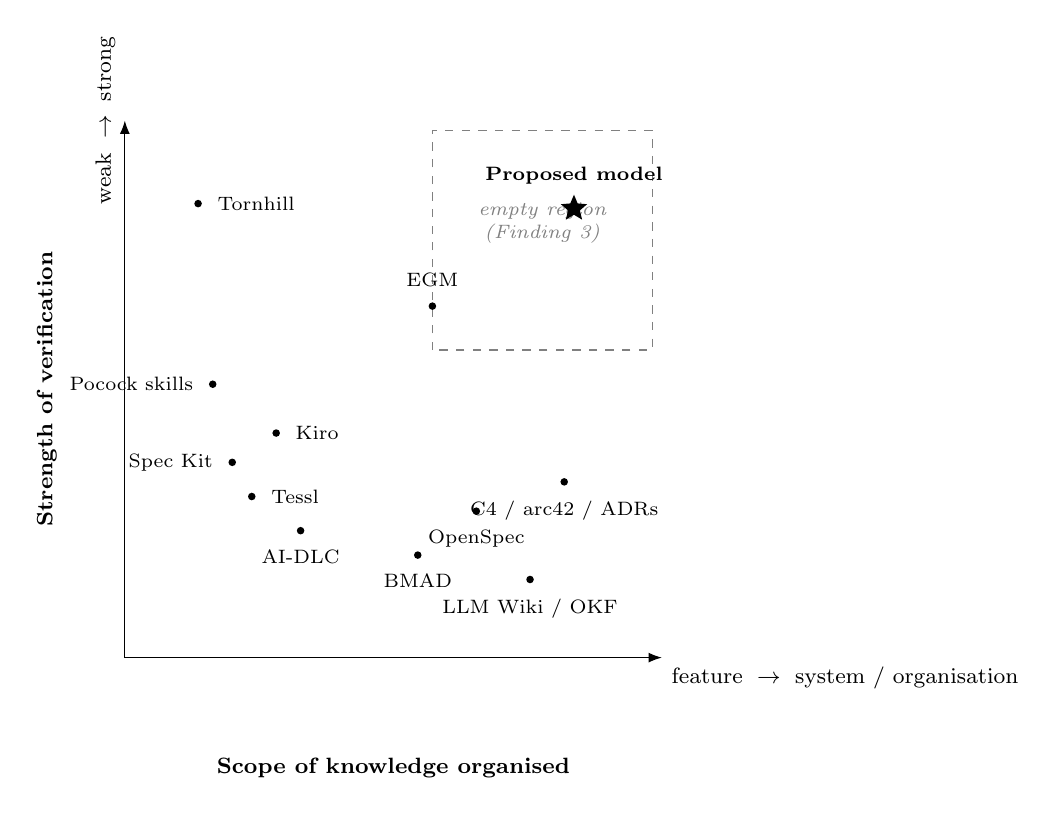
\begin{tikzpicture}[scale=0.62]
  % axes
  \draw[-{Latex}] (0,0) -- (11,0) node[below right, font=\footnotesize] {feature $\;\to\;$ system / organisation};
  \draw[-{Latex}] (0,0) -- (0,11) node[above left, font=\footnotesize, rotate=90, anchor=south] {weak $\;\to\;$ strong};
  \node[below=10pt, font=\footnotesize\bfseries] at (5.5,-1.3) {Scope of knowledge organised};
  \node[rotate=90, font=\footnotesize\bfseries] at (-1.6,5.5) {Strength of verification};

  % empty upper-right region the proposed model targets
  \draw[dashed, gray] (6.3,6.3) rectangle (10.8,10.8);
  \node[align=center, font=\scriptsize\itshape, text=gray] at (8.55,8.9) {empty region\\(Finding 3)};

  % reviewed techniques (qualitative positions; author's assessment)
  \fill (1.5,9.3) circle (2.2pt); \node[right, font=\scriptsize] at (1.7,9.3) {Tornhill};
  \fill (6.3,7.2) circle (2.2pt); \node[above, font=\scriptsize] at (6.3,7.4) {EGM};
  \fill (9.0,3.6) circle (2.2pt); \node[below, font=\scriptsize] at (9.0,3.4) {C4 / arc42 / ADRs};
  \fill (7.2,3.0) circle (2.2pt); \node[below, font=\scriptsize] at (7.2,2.8) {OpenSpec};
  \fill (6.0,2.1) circle (2.2pt); \node[below, font=\scriptsize] at (6.0,1.9) {BMAD};
  \fill (8.3,1.6) circle (2.2pt); \node[below, font=\scriptsize] at (8.3,1.4) {LLM Wiki / OKF};
  \fill (3.6,2.6) circle (2.2pt); \node[below, font=\scriptsize] at (3.6,2.4) {AI-DLC};
  \fill (1.8,5.6) circle (2.2pt); \node[left, font=\scriptsize] at (1.6,5.6) {Pocock skills};
  \fill (3.1,4.6) circle (2.2pt); \node[right, font=\scriptsize] at (3.3,4.6) {Kiro};
  \fill (2.2,4.0) circle (2.2pt); \node[left, font=\scriptsize] at (2.0,4.0) {Spec Kit};
  \fill (2.6,3.3) circle (2.2pt); \node[right, font=\scriptsize] at (2.8,3.3) {Tessl};

  % proposed model
  \node[star,star points=5,star point ratio=2.2,fill=black,inner sep=1.6pt] at (9.2,9.2) {};
  \node[above, font=\scriptsize\bfseries] at (9.2,9.5) {Proposed model};
\end{tikzpicture}
\caption{Qualitative position of the 11 reviewed techniques and the proposed model on two axes: the scope of knowledge a technique organises, and the strength with which it verifies what was written. Positions are the author's qualitative assessment (Section 10), not a measurement. The upper-right region is empty: techniques that verify well (Tornhill) operate at feature scope, and techniques that organise system-level knowledge (C4, OpenSpec, LLM Wiki/OKF) verify weakly. The model proposed in Section 7 targets the empty region.}
\label{fig:positioning}
\end{figure}

The upper-right region is empty. Techniques that verify well operate at feature scope; those that organise system-level or organisation-level knowledge barely verify. The model proposed in Section 7 targets that region.

% ==========================================================================
\section{Results III: knowledge directory structures}

How files are organised looks like an implementation detail, but it decides what an agent can find unaided and what is lost over time. The reviewed techniques use seven organising axes, each answering some questions well and others poorly.

\small
\begin{longtable}{p{0.2\linewidth}p{0.2\linewidth}p{0.27\linewidth}p{0.27\linewidth}}
\caption{Organising axes of knowledge directories.}\\
\toprule
\textbf{Axis} & \textbf{Examples} & \textbf{Answers well} & \textbf{Answers poorly} \\
\midrule
\endfirsthead
\toprule
\textbf{Axis} & \textbf{Examples} & \textbf{Answers well} & \textbf{Answers poorly} \\
\midrule
\endhead
By feature & Spec Kit, Kiro specs & What should this feature do? & What is the system like after twenty features? \\
By change, with current truth separate & OpenSpec & What changes now, and what is current behaviour? & How is the system divided, and why? \\
By phase and intent & AI-DLC & What was decided at each stage, and by whom? & Where is current knowledge about a component? \\
By document type & BMAD & Which is the PRD, which is the architecture? & Which part of the architecture does this code implement? \\
By concept & LLM Wiki, OKF & What do we know about this topic? & Where is it in the code? \\
By code directory & EGM bootstrap & What does this directory do, and what is its contract? & Why was it divided this way? \\
By architecture element & C4 as DSL & What are the parts and who talks to whom? & What behaviour is expected of each part? \\
\bottomrule
\end{longtable}
\normalsize

\subsection{The EGM structure}

EGM combines two axes. Design documents live in \texttt{docs/designs/}, indexed by a sitemap. The more original idea is in its bootstrap skill, which the project calls ``peanuts and hay''. Peanuts are README files in leaf directories holding per-file contracts: interfaces, invariants, and side effects. Hay is the set of parent READMEs that roll child contracts up into progressively higher-altitude indexes, until the root becomes a map of the system's architecture (\href{https://github.com/google/elephant-goldfish-model/blob/main/skills/egm_bootstrap/SKILL.md}{egm\_bootstrap}). Generated content sits inside sentinel blocks so that human-written text is preserved.

Five properties make this structure especially relevant to agent-assisted work:

\begin{enumerate}[leftmargin=*]
  \item \textbf{Co-location.} Knowledge about a directory lives in that directory. An agent opening the code finds the contract without searching, and a change to code and contract fits in one pull request.
  \item \textbf{Emergent zoom.} The README hierarchy reproduces the zoom levels of C4 without anyone drawing them: leaf as component, intermediate as container, root as system.
  \item \textbf{Contracts, not descriptions.} Interfaces, invariants, and side effects are the knowledge most useful for implementation and easiest to verify against code.
  \item \textbf{Provenance.} Sentinel blocks separate machine-generated from human-written content.
  \item \textbf{Checkable by a goldfish.} Because everything is linked by files, a zero-context subagent can navigate the hierarchy; what it cannot reach is not written down.
\end{enumerate}

\subsection{Where it falls short}

The physical folder tree is not the logical architecture: cross-cutting concerns, components spread across folders, and systems split across repositories do not fit a directory hierarchy. Contracts say what, not why; decisions and discarded alternatives have no place in a component README. And automatic bottom-up generation runs exactly the risk Storey calls automation of understanding; EGM itself notes that humans still need to review the output.

\textbf{Finding 4 (RQ1): no single axis suffices.} The strongest structure combines four: current truth separated from changes (OpenSpec), contracts co-located with code (EGM), a logical model that cuts across folders (C4), and a linked base of concepts and decisions (OKF).

The weakness of the by-feature axis has an empirical precedent. In large-scale agile programmes, teams working from some 2,000 user stories struggled to describe the complete system and fell back on epics and themes to regain an overview (Kasauli et al., 2021, as reviewed by Sporsem et al., 2026). Feature-scoped specification kits reproduce the same structure, at agent speed.

% ==========================================================================
\section{The Bounded Delegation model}

This section answers RQ3. The four findings point to the same gap: techniques either bound the agent's work with prose that nobody can execute, or with tests that carry no rationale, and none keeps people's understanding in the loop by design. The model below combines the strongest element of each reviewed approach around the central hypothesis $H_0$ (Section 1.2).

\subsection{Sub-hypotheses}

$H_0$ decomposes into six sub-hypotheses. Each states a comparison and a predicted direction, so that each can fail independently.

\small
\begin{longtable}{p{0.05\linewidth}p{0.22\linewidth}p{0.28\linewidth}p{0.2\linewidth}}
\caption{Sub-hypotheses of the Bounded Delegation model.}\\
\toprule
\textbf{ID} & \textbf{Hypothesis} & \textbf{Prediction} & \textbf{Derived from} \\
\midrule
\endfirsthead
\toprule
\textbf{ID} & \textbf{Hypothesis} & \textbf{Prediction} & \textbf{Derived from} \\
\midrule
\endhead
H1 & \textbf{Boundary reading.} Humans who read intent and inspectable scenarios, and read implementation only by exception, detect behavioural defects at least as well as humans who review implementation line by line. & Equal or lower escaped-defect rate, with lower human review time per change & Tornhill; DORA on verification cost \\
H2 & \textbf{Executable bound.} Locked, inspectable scenarios written before implementation reduce behaviour drift relative to prose specifications. & Fewer divergences between stakeholder expectation and observed behaviour & Tornhill; Farley; Finding 3; Carlile (semantic boundary) \\
H3 & \textbf{Context-free verification.} Artifacts that pass zero-context review require fewer agent clarifications and less rework than artifacts reviewed by context-rich reviewers. & Fewer clarification requests and fewer tokens per change & EGM; Storey on intent debt \\
H4 & \textbf{Structured context.} Co-located contracts linked to an explicit architecture model reduce architecture violations and context cost compared with feature-scoped specifications alone. & Fewer violated architectural assertions; fewer files read per change & EGM; C4; Finding 4 \\
H5 & \textbf{Feedback.} Per-layer feedback from evidence back to intent slows the growth of artifact staleness and model-code drift. & Lower drift and artifact age over 6 to 12 months & OpenSpec; Lehman; Finding 1; Sporsem et al.\ (P5) \\
H6 & \textbf{Attention as the constraint.} Limiting pending human decisions per person predicts delivery stability better than time-boxed, velocity-based planning. & Lower change failure rate at equal throughput & DORA; Finding 2 \\
\bottomrule
\end{longtable}
\normalsize

If H1 fails, humans must keep reading implementation and the model's economy collapses. If H3 fails, isolated review is cost without benefit. The hypotheses are deliberately separable.

The evidential basis is uneven, and we state it plainly. By the threshold Sporsem et al.\ (2026) apply, at least three distinct empirical sources per proposition, none of the six qualifies yet. H1, H5, and H6 draw on at least one peer-reviewed or large-survey source (DORA; Lehman), while H2, H3, and H4 rest mainly on practitioner reports and on this review's own findings. All six are therefore conjectures to be tested, not propositions synthesised from evidence.

\subsection{Seven knowledge layers}

The model organises knowledge in seven layers. Layers 1--3 form the \emph{intent bound}; layer 7 is the \emph{evidence bound}; layers 4--6 are the delegated path.

\begin{enumerate}[leftmargin=*]
  \item \textbf{Problem.} Who is affected, what counts as success, constraints, and quality scenarios. \emph{Humans decide.}
  \item \textbf{Domain.} The business language, term by term. \emph{Humans decide.}
  \item \textbf{Decisions.} ADRs with machine-checkable assertions. \emph{Humans decide.}
  \item \textbf{Structure.} A C4 model linked to component contracts in the code.
  \item \textbf{Patterns.} Recurring solutions with implementation steps.
  \item \textbf{Steps.} Changes in progress, with deltas over the layers above.
  \item \textbf{Evidence.} Inspectable executable scenarios, architecture tests, and evaluations. \emph{Humans read; agents may not edit.}
\end{enumerate}

Layer 7 is not written last. Executable scenarios are drafted right after the problem, before any step, and they, rather than a prose document, are the specification the agent must satisfy. The prose of layers 1--3 keeps what tests cannot say: the rationale.

Rationale has a cost, and the model must place it where it is paid once. Stating the ``why'' focuses work on user needs, but the true reason often takes several rounds of asking, and developers omitted it when the same reason applied to many stories (Sporsem et al., 2026, P3; Diebold et al., 2018). The layering answers this: a reason that holds for many increments is written once, in layer 1 or 3, and each increment links to it instead of restating it. Technical requirements with no user to speak for them go to decisions, not to scenarios, much as Kniberg (2015) kept tech stories apart from user stories.

Scenarios alone are not a specification. Meyer's (2018) criticism of user stories applies to them unchanged: piling up case over case does not give a specification, only a system that handles the planned cases and possibly nothing else. This is why layer 7 is bounded from above by layers 1--4: quality scenarios, decisions, and structure state the general properties that no list of cases implies. Non-functional requirements are the clearest gap. User stories handled them poorly (Behutiye et al., 2020), and end-to-end scenarios inherit that weakness unless the quality scenarios of layer 1 are turned into checks.

\subsection{Three roles}

From EGM the model takes its second rule: authors do not verify their own artifacts. \textbf{Elephants} receive maximal context and draft. \textbf{Goldfish} receive none: only the artifact, the files it links to, and the code. \textbf{Humans} decide the premises in layers 1--3 and, before approving, explain the change in their own words. The goldfish measures intent debt (is the artifact self-sufficient?); the human explanation measures cognitive debt (does the team understand it?). Neither test replaces the other.

The human role has a name in boundary object theory. Levina and Vaast (2005) call \emph{boundary spanners} the people who adapt objects to each side, show others how to use them, and introduce them at the right time. In agile requirements engineering, a story's effect depended more on the skill of the person writing and telling it than on the story itself (Sporsem et al., 2026, P1; Conboy, 2021). Under bounded delegation, keeping the bounds legible to both people and agents is that spanning work: a skill to be valued when staffing a team, not a by-product of approving changes.

\subsection{The iterative and incremental cycle}

Each increment is a thin, complete slice of behaviour, small enough to be understood at once and delivered in hours or a few days. The cycle alternates between humans and agents, and humans appear at four bounds.

\begin{figure}[htbp]
\centering
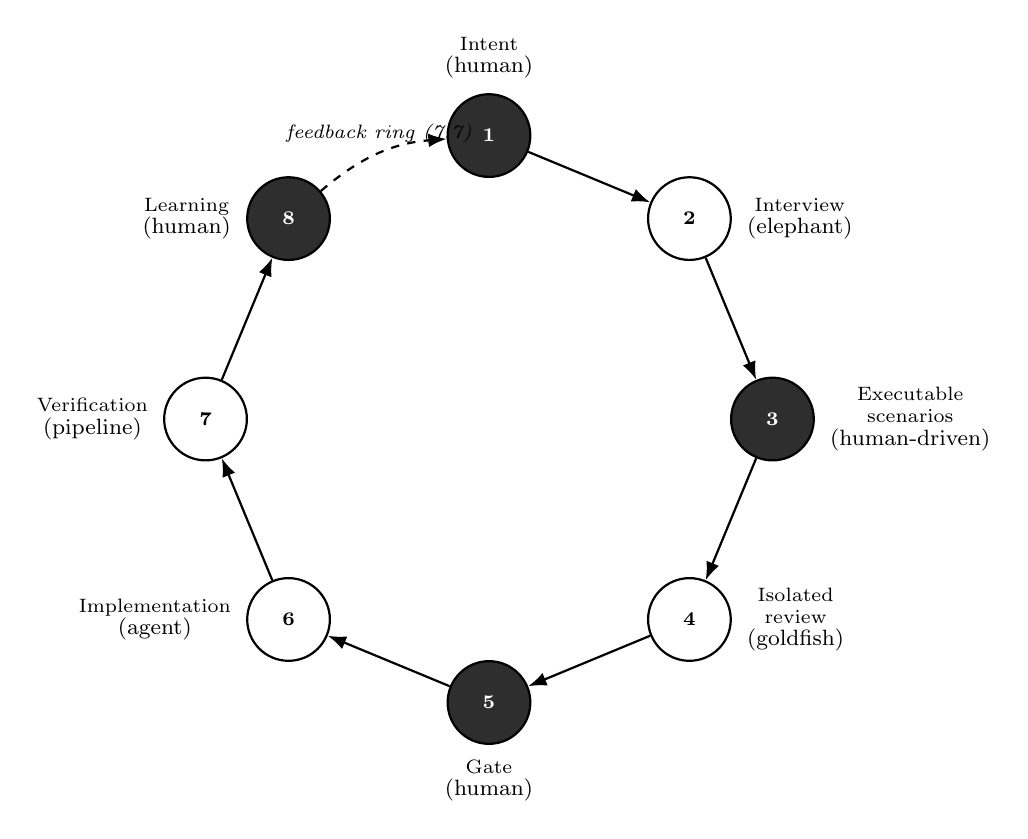
\begin{tikzpicture}[
  scale=1,
  stepnode/.style={circle, minimum size=1.05cm, inner sep=0pt, font=\scriptsize\bfseries, draw, thick},
  human/.style={stepnode, fill=black!82, text=white},
  agent/.style={stepnode, fill=white, text=black},
  lbl/.style={font=\scriptsize, align=center}
]
  % 8 nodes evenly spaced on a circle, step 1 at top, clockwise
  \def\R{3.6}
  \node[human] (s1) at (90:\R)  {1};
  \node[agent] (s2) at (45:\R)  {2};
  \node[human] (s3) at (0:\R)   {3};
  \node[agent] (s4) at (-45:\R) {4};
  \node[human] (s5) at (-90:\R) {5};
  \node[agent] (s6) at (-135:\R){6};
  \node[agent] (s7) at (180:\R) {7};
  \node[human] (s8) at (135:\R) {8};

  % cycle arrows
  \draw[-{Latex}, thick] (s1) -- (s2);
  \draw[-{Latex}, thick] (s2) -- (s3);
  \draw[-{Latex}, thick] (s3) -- (s4);
  \draw[-{Latex}, thick] (s4) -- (s5);
  \draw[-{Latex}, thick] (s5) -- (s6);
  \draw[-{Latex}, thick] (s6) -- (s7);
  \draw[-{Latex}, thick] (s7) -- (s8);
  \draw[-{Latex}, thick, dashed] (s8) to[bend left=18] node[midway, above, font=\scriptsize\itshape] {feedback ring (7.7)} (s1);

  % labels outside each node
  \node[lbl, above=2pt of s1] {Intent\\\footnotesize(human)};
  \node[lbl, right=2pt of s2] {Interview\\\footnotesize(elephant)};
  \node[lbl, right=2pt of s3] {Executable\\scenarios\\\footnotesize(human-driven)};
  \node[lbl, right=2pt of s4] {Isolated\\review\\\footnotesize(goldfish)};
  \node[lbl, below=2pt of s5] {Gate\\\footnotesize(human)};
  \node[lbl, left=2pt of s6] {Implementation\\\footnotesize(agent)};
  \node[lbl, left=2pt of s7] {Verification\\\footnotesize(pipeline)};
  \node[lbl, left=2pt of s8] {Learning\\\footnotesize(human)};
\end{tikzpicture}
\caption{One increment under Bounded Delegation: 8 steps, alternating human bounds (filled nodes: Intent, Executable scenarios, Gate, Learning) and agent-performed steps (outlined nodes: Interview, Isolated review, Implementation, Verification). The dashed arrow closes the feedback ring described in Section 7.7, which routes drift signals from evidence back up to intent.}
\label{fig:cycle}
\end{figure}

\begin{enumerate}[leftmargin=*]
  \item \textbf{Intent.} A person states the problem, the motivation, and known constraints.
  \item \textbf{Interview.} An elephant with system context asks until gaps close; new terms go to the glossary, and a structural decision becomes a draft ADR.
  \item \textbf{Executable scenarios.} The person drives, with the agent, the end-to-end tests of the increment, makes them readable in domain language, and commits the suite. From here, implementing agents cannot change it.
  \item \textbf{Isolated review.} Goldfish read the scenarios and the layer deltas without the conversation and report what does not stand alone.
  \item \textbf{Gate.} The person approves what is premise and explains the change back.
  \item \textbf{Implementation.} Agents implement in small batches, each in an ephemeral workspace, integrating to trunk behind a feature flag when the increment is incomplete.
  \item \textbf{Verification.} The pipeline runs the locked scenarios, the architecture tests, automated reviews, and model-code comparison. Failures return to step 6 without human involvement.
  \item \textbf{Learning.} The person reads results (scenarios, production metrics, feedback signals) and adjusts the intent of the next increment.
\end{enumerate}

The evidence on user stories supports this size. Small stories were estimated more accurately, exposed dependencies earlier, and shortened the wait for user feedback; large ones grew unexpectedly and produced more code than needed (Liskin et al., 2014, as reviewed by Sporsem et al., 2026, P2). Small items also gave developers short-term certainty inside long-term uncertainty, which Vidgen and Wang (2009) relate to Baskerville's (2006) ``artful planning''. The same review warns that the benefit fades at scale, where many small items must be regrouped to keep an overview; in the model that regrouping belongs to layers 1 and 4, not to the increment.

The cycle formalises what practitioners already report doing. Karpathy describes the same alternation as a generation-verification loop to be spun as fast as possible in small chunks. Horthy places the human checkpoints on research and plans rather than on code. Cherny names the agent's ability to verify its own work as the practice that matters most. The model adds two things those accounts leave implicit: that the verification artifact is owned and locked by a person, and that the reviewer of each artifact starts without context.

\subsection{What humans read and what agents read}

\small
\begin{longtable}{p{0.22\linewidth}p{0.37\linewidth}p{0.33\linewidth}}
\caption{Relevance of each element to humans and to agents.}\\
\toprule
\textbf{Element} & \textbf{For humans} & \textbf{For agents} \\
\midrule
\endfirsthead
\toprule
\textbf{Element} & \textbf{For humans} & \textbf{For agents} \\
\midrule
\endhead
Problem, goal, constraints & Write and decide; revisit with production metrics & Read as a limit; never alter \\
Domain language & Choose the terms & Use in names, tests, and messages \\
Decisions (ADRs) & Weigh alternatives, decide, be able to explain & Obey assertions; propose revision when a signal repeats \\
Executable scenarios & \textbf{Primary reading}: drive, check, lock & Implement until they pass; editing forbidden \\
C4 model & Read context and containers; review model diffs & Read components; navigate; propose changes \\
Co-located contracts & Review by sampling & Primary context when touching code \\
Patterns and skills & Curate & Execute \\
Implementation code & Read by exception: hotspots, failures, incidents & Write and keep healthy \\
Quality and architecture thresholds & Define & Meet, under automatic verification \\
Feedback log and signals & Decide the response; lead understanding practices & Detect, record, propose \\
\bottomrule
\end{longtable}
\normalsize

The rule that summarises the table is the hypothesis restated operationally: \textbf{humans read intent and evidence; agents read and write the path between them.}

\subsection{Repository structure}

The structure combines the four axes of Finding 4.

\begin{verbatim}
.
|-- AGENTS.md                    # router: what to read, in which order
|-- CONTEXT.md                   # layer 2: domain language
|-- knowledge/                   # OKF bundle: current truth
|   |-- index.md   log.md        # catalogue and feedback trail
|   |-- problem/                 # layer 1
|   |-- decisions/               # layer 3: ADRs
|   `-- patterns/                # layer 5
|-- architecture/
|   |-- workspace.dsl            # layer 4: C4 model
|   `-- SITEMAP.md               # generated: C4 element -> README -> changes
|-- changes/                     # layer 6: one folder per increment
|   |-- 2026-11-rescheduling/
|   |   |-- proposal.md  tasks.md
|   |   |-- deltas/              # what changes in layers 1 to 5
|   |   `-- reviews/             # goldfish reports
|   `-- archive/
|-- tests/
|   |-- acceptance/              # layer 7: executable scenarios (locked)
|   `-- architecture/            # layer 7: ADR assertions
|-- src/scheduling/
|   `-- README.md                # component contract
`-- .agents/skills/
\end{verbatim}

The \texttt{tests/acceptance/} folder carries its own rule: the implementing agent has no write permission there. The lock is enforced by the environment, not requested in the prompt.

\subsection{The feedback ring}

Each layer returns a signal to the one above when reality contradicts it: a failing test creates a new step; repeated steps become a pattern; a pattern that does not fit changes the model; recurring model-code drift reopens a decision; a decision that meets an ambiguous term returns to the glossary; the domain may show that the problem was a different one. The top layer closes the ring by returning new scenarios to the evidence layer. Returns slow down as they rise, so that the system does not oscillate, and each leaves a line in \texttt{log.md}.

Not every artifact must be kept current. Sporsem et al.\ (2026, P5) find that written user stories degrade once implemented and ask whether this is a problem at all, since the story has served its purpose. The model accepts that answer for layer 6: a change folder is a reminder of a conversation, and it is archived rather than maintained. It rejects it for layers 1--5 and 7, which agents read as current truth in every session. A stale story misleads one newcomer once; a stale contract misleads every agent run. The ring therefore applies only to the layers that are read as current.

Alongside artifact sensors, the ring has sensors for cognitive debt, taken from Storey's diagnostic signals: changes with unexpected results, components nobody wants to touch, knowledge concentrated in one person. The response to these is never a generated document. It is a human practice: an explanation, a walkthrough, a pairing session.

Agile teams already had such a practice. In a longitudinal case, developers working in rotating pairs spread their understanding of user needs well beyond what the written stories held (Vidgen and Wang, 2009). Rotation can survive when agents write the code: the pair's task becomes reading the bounds together and explaining a change to each other.

\subsection{Code that both readers understand}

If humans read implementation only by exception, do Clean Code and Clean Architecture still matter? The principles matter more; the ceremony matters less. Borg et al. (2026) found an association between code health, a metric calibrated for human comprehension, and behaviour preservation after AI refactoring, though on small, isolated files.

\small
\begin{longtable}{p{0.3\linewidth}p{0.22\linewidth}p{0.4\linewidth}}
\caption{Code design practices under bounded delegation.}\\
\toprule
\textbf{Practice} & \textbf{Recommendation} & \textbf{Reason} \\
\midrule
\endfirsthead
\toprule
\textbf{Practice} & \textbf{Recommendation} & \textbf{Reason} \\
\midrule
\endhead
Names in domain language & Keep & Agents infer purpose from names, as people do \\
Low complexity, cohesion, no duplication & Keep, with a pipeline threshold & What health metrics measure and what correlates with correct changes \\
Dependency rule (domain ignores infrastructure) & Keep, as an architecture test & Limits the reach of each change and is machine-checkable \\
Ports and adapters & Keep & An obvious place for each thing; testable without infrastructure \\
Deep modules with small interfaces & Strengthen & Fewer files and hops to understand a behaviour (Ousterhout, 2021) \\
Vertical slices by feature & Strengthen & Keeps together what changes together, with the contract beside the code \\
Tiny functions, one class per concept & Reduce & Spreads one behaviour over dozens of files and consumes context \\
An interface for every class; DTOs and mappers between all layers & Reduce & Cheap for agents to write, costly for everyone to read \\
Folders by technical layer only & Avoid & Separates what changes together \\
``Good code needs no comments'' & Revise & Code says what; the why belongs in ADRs and contracts \\
\bottomrule
\end{longtable}
\normalsize

The criterion for any abstraction becomes a single question: does it reduce what a human and an agent must read to change something safely?

\subsection{The bounds as boundary objects}

Read through boundary object theory (Section 2.6), the model's human-owned layers are boundary objects between people and agents, and each addresses one of Carlile's (2002) knowledge boundaries (Table~\ref{tab:boundaries}).

\small
\begin{longtable}{p{0.12\linewidth}p{0.28\linewidth}p{0.22\linewidth}p{0.28\linewidth}}
\caption{Carlile's knowledge boundaries between people and agents.}\label{tab:boundaries}\\
\toprule
\textbf{Boundary} & \textbf{What goes wrong between people and agents} & \textbf{Layer that carries it} & \textbf{Check in the model} \\
\midrule
\endfirsthead
\toprule
\textbf{Boundary} & \textbf{What goes wrong between people and agents} & \textbf{Layer that carries it} & \textbf{Check in the model} \\
\midrule
\endhead
Syntactic & The agent uses words the team does not use, or invents names & 2. Domain (glossary) & Names in domain language; goldfish flag undefined terms \\
Semantic & The agent reads the same words differently from the team & 7. Evidence (executable scenarios) & A scenario passes or fails; a second reading cannot pass silently \\
Pragmatic & Interests conflict: speed against structure, one team's change against another's & 3. Decisions (ADRs) and the human gate & People decide; agents propose a revision when a signal repeats \\
\bottomrule
\end{longtable}
\normalsize

Two consequences follow. First, an executable scenario crosses the semantic boundary in a way a user story could not. The story left meaning to a later conversation; a scenario fixes it in a form that a person and an agent check the same way. This is the strongest theoretical reason for H2. Second, the pragmatic boundary cannot be delegated. Carlile holds that crossing it requires the parties to transform their knowledge and to be able to alter the object; an agent can propose, but the trade-off between interests stays with people. This is why layers 1--3 are human-owned.

Levina and Vaast's (2005) distinction gives a test for the gate. An approved artifact that nobody reads again is a designated boundary object, not one in use, and repeated approval without reading (Section 4.2, AI-DLC) produces exactly that. The explain-back at the gate and the goldfish review exist to keep the bounds in use. H5's measure of artifact age is, in these terms, a measure of how long a bound stays in use. Sporsem et al.'s (2026) open questions on how people and language models read the same requirement at each boundary map onto H2 (semantic) and H3 (syntactic) of this agenda.

The theory also names a tension the model must hold. Crossing a pragmatic boundary requires interpretive flexibility: an object each group can read from its own interests while it stays a common reference (Star, 2010; Doolin and McLeod, 2012). An executable scenario removes that flexibility by design. The model therefore keeps the two properties in different layers: the prose of layers 1--3 stays open to negotiation; the scenarios of layer 7 are closed to implementing agents from step 3 of the cycle (Section 7.4) but stay open to people until the gate at step 5, where the negotiation ends. Treating a scenario as final before the pragmatic boundary is crossed would turn one group's reading into everyone's constraint. Boundary objects are also in use only for periods (Sporsem et al., 2026): a bound that people have stopped reading has become a designated object again, whatever its age.

% ==========================================================================
\section{Contrast with the software engineering canon}

This section answers RQ4 by contrasting the model with the traditional literature. It proceeds from the general to the specific: the fundamentals stated by the textbooks and the body of knowledge (8.1), the values of the Agile Manifesto (8.2), the current positions of its authors (8.3), the process practices built on those foundations (8.4), and the recommendations that follow (8.5). The overall result is that the foundations hold and their allocation changes.

\subsection{Fundamentals preserved and fundamentals that change}

Read against the canon of Section 2.4, bounded delegation is conservative about what software engineering is and radical about who does which part of it. Table~\ref{tab:canon} contrasts each fundamental with its fate under the hypothesis.

\small
\begin{longtable}{p{0.24\linewidth}p{0.17\linewidth}p{0.4\linewidth}p{0.11\linewidth}}
\caption{Fundamentals of the canon under bounded delegation.}
\label{tab:canon}\\
\toprule
\textbf{Fundamental} & \textbf{Canonical source} & \textbf{Under bounded delegation} & \textbf{Verdict} \\
\midrule
\endfirsthead
\toprule
\textbf{Fundamental} & \textbf{Canonical source} & \textbf{Under bounded delegation} & \textbf{Verdict} \\
\midrule
\endhead
Essence and accident: the hard part is the conceptual construct, not its representation & Brooks (1987) & Agents absorb accidental work; the essence (what to build, and why) becomes the whole of the human task & Preserved, and made visible \\
Four fundamental activities: specification, development, validation, evolution & Sommerville (2016) & All four remain. Specification and validation become the human-owned bounds; development is delegated; evolution is shared through feedback & Preserved, redistributed \\
Quality focus as the bedrock of the discipline & Pressman and Maxim (2020) & Remains the base, but is enforced by machine thresholds rather than by review discipline & Preserved, mechanised \\
Layered technology: process, methods, tools & Pressman and Maxim (2020) & The top layer changes nature: tools no longer support the methods, they execute construction & Transformed \\
Construction as the bulk of effort & SWEBOK construction area (Washizaki, 2024); Pressman's framework & Construction becomes the cheapest activity; requirements, architecture, and testing absorb the human effort & Inverted \\
Information hiding and modularity & Parnas (1972) & More important: module boundaries bound the context an agent must read and the reach of a wrong change & Strengthened \\
Software evolves and degrades unless work is done against it & Lehman (1980) & Holds at higher speed; drift appears in weeks, not years & Preserved, accelerated \\
Cost of change rises through the life cycle & Boehm (1981); flattened by short loops in Beck (1999) & Changing code becomes cheap at any stage. Changing a wrong decision or a misunderstood intent stays expensive & Split: holds for intent, not for code \\
Effort estimation from size and person-months & Boehm (1981) & Loses its basis when implementation time is small and variable; the constraint is human attention & Weakened \\
Code is written for people to read & Martin (2008); Fowler (2018) & Implementation is read mostly by agents; people read scenarios, contracts, and decisions & Transformed \\
Technical review and inspection of code by people & Pressman and Maxim (2020) & Line-by-line review gives way to boundary reading and automated review; human review persists at hotspots & Transformed \\
Programming as theory building & Naur (1985) & The theory must now be written, because the main executor holds none & Preserved, endangered \\
\bottomrule
\end{longtable}
\normalsize

Three observations follow from the table.

First, the hypothesis is Brooks's argument restated for a new tool. Brooks predicted that attacking accidental complexity would never deliver an order-of-magnitude gain in the whole, because the essence would remain. Agents are the most powerful attack on accident so far, and the empirical record of Section 2.2, with large individual speed-ups and flat team outcomes, is what Brooks's argument predicts. The two bounds of the model are the essence in his sense: deciding what the construct should be, and establishing that the construct built is the one intended.

Second, Sommerville's four activities survive intact, and this is the strongest evidence that the discipline's foundations are not being replaced. What changes is their allocation. In the textbook account one team performs all four. Under bounded delegation, people hold specification and validation, agents hold development, and evolution is a loop between them.

Third, the single fundamental that changes in kind is the readership of code. The canon's craft literature, from Martin's \emph{Clean Code} to Fowler's \emph{Refactoring}, assumes that the primary reader of a program is another programmer. Section 7.8 argued that the practices this literature recommends still pay off, because code that is healthy for people is also safer for agents to change. But the reason shifts, from courtesy to a future colleague to a property that machines can measure and enforce.

\subsection{The Agile Manifesto revisited}

The Manifesto (Beck et al., 2001) is often read as a rejection of documentation and process. Its text is a set of preferences, and each can be re-read with agents as the main implementers.

\small
\begin{longtable}{p{0.24\linewidth}p{0.24\linewidth}p{0.34\linewidth}p{0.1\linewidth}}
\caption{The four values of the Agile Manifesto under bounded delegation.}\label{tab:manifesto}\\
\toprule
\textbf{Value} & \textbf{Original concern} & \textbf{Reading under bounded delegation} & \textbf{Verdict} \\
\midrule
\endfirsthead
\toprule
\textbf{Value} & \textbf{Original concern} & \textbf{Reading under bounded delegation} & \textbf{Verdict} \\
\midrule
\endhead
Individuals and interactions over processes and tools & Heavy process displaced the judgement of the people doing the work & The tool is now a participant. Interactions among people become the scarce resource, since that is where understanding is built; agent throughput must not crowd them out & Preserved, with higher stakes \\
Working software over comprehensive documentation & Documents were treated as progress in place of software & Working software remains the measure. But an agent has no tacit knowledge, so recorded intent is no longer optional. Inspectable executable scenarios reconcile the two: they are documentation that runs & Preserved, rebalanced \\
Customer collaboration over contract negotiation & Fixed requirements froze learning & Cheap increments make collaboration more frequent; the interview at the start of each increment is collaboration by design & Strengthened \\
Responding to change over following a plan & Plans outlived the facts they were based on & Code change is cheap, so responsiveness rises. The plan that must now respond is the set of intent artifacts, which is why the model needs a feedback ring & Strengthened, extended to intent \\
\bottomrule
\end{longtable}
\normalsize

Several of the twelve principles shift in the same way. ``Working software is the primary measure of progress'' holds unchanged. ``Continuous attention to technical excellence and good design enhances agility'' gains empirical support from the code-health evidence. ``Simplicity, the art of maximising the amount of work not done'' becomes more important, because an agent's default is to produce more. ``Sustainable pace'' re-appears as a limit on pending human decisions (H6). The principle that face-to-face conversation is the most effective way to convey information needs qualification: it remains true among people, but an agent was not in the room, so the outcome of the conversation has to be written down before it can guide the work. Sedano, Ralph, and P\'eraire (2019) state the tension precisely: a good specification replaces face-to-face communication, while a good backlog facilitates it. Bounded delegation needs both. The bounds replace conversation for the agent, and must not replace it among people.

Cockburn's (2006) description of development as a cooperative game of invention and communication survives well. The game now has a new kind of player, one that communicates only through written artifacts and remembers nothing between sessions. Much of the model in Section 7 is a response to that single property.

The Extreme Programming practices fare differently from one another. Test-driven development moves from a programmer's technique to the contract between people and agents. Continuous integration and small releases become preconditions rather than aspirations. Refactoring is delegated but not diminished. Pair programming changes most: pairing with an agent keeps the productivity benefit but loses the function Beck (1999) valued most, the spreading of knowledge between two people, which is why the model replaces it with explicit understanding practices rather than assuming it away. Hunt and Thomas's (1999) tracer bullets, thin end-to-end slices that prove the architecture, are the increments of Section 7.4 almost unchanged.

\subsection{What the canon's authors say now}

Three signatories of the Manifesto have published their own positions on working with agents, and they do not fully agree, which is informative for H1.

\textbf{Beck} distinguishes \emph{augmented coding} from vibe coding. In the former the developer still cares about the code, its complexity, its tests, and their coverage; the value system is that of hand coding, with less typing. He reports abandoning two attempts at a project because accumulated complexity stalled the agent, and treats test-driven development as the way to keep it on course (\href{https://newsletter.kentbeck.com/p/augmented-coding-beyond-the-vibes}{Beck, 2025}).

\textbf{Fowler} argues that LLMs change programming as much as the move from assembler to high-level languages did, with a difference: the new abstraction is non-deterministic, a sideways move rather than only an upward one (\href{https://martinfowler.com/articles/2025-nature-abstraction.html}{Fowler, 2025}). He suggests that software engineering will need the notion of tolerances that other engineering disciplines use, and that rigorous testing and refactoring matter more, not less (\href{https://thenewstack.io/martin-fowler-on-preparing-for-ais-nondeterministic-computing/}{The New Stack}; \href{https://newsletter.pragmaticengineer.com/p/martin-fowler}{The Pragmatic Engineer}). He also notes that developers usually gain their understanding of a domain and a system in the act of building it, which is the mechanism behind cognitive debt (\href{https://www.martinfowler.com/fragments/2026-02-09.html}{Fowler, 2026}).

\textbf{Martin}, whose \emph{Clean Code} taught a generation to write for human readers, reported in 2026 that he no longer reads the code his agents write. He surrounds them instead with constraints: unit tests, Gherkin acceptance tests, QA procedures, complexity and module-size thresholds, dependency analysis, mutation testing, and coverage (\href{https://startupfortune.com/?p=16790}{Startup Fortune}; \href{https://noqta.tn/en/blog/disciplined-agentic-engineering-uncle-bob-tdd-ai-2026}{Noqta}). Secondary reports add that he continues to draw module boundaries himself.

These positions map onto the model. Martin's practice and Tornhill's are, independently, the boundary-reading stance of H1: people own acceptance tests and structure, machines check everything else. Beck's position keeps the human closer to the code. Fowler's concern with non-determinism explains why the evidence bound must be executable and locked: a prose specification interpreted by a non-deterministic tool gives no stable guarantee. The disagreement between Beck and Martin is the open empirical question that H1 is designed to settle, and it is notable that it now divides authors who agreed on almost everything in 2001.

\subsection{Practices that lose their rationale}

If the fundamentals hold, why should practices change? Because much of the development process of the last two decades was designed to ration one scarce resource: programmer hours. When implementation takes minutes, the scarce resource becomes human attention for deciding, checking, and understanding. Practices that existed to manage the first lose their rationale, while the principles beneath them gain importance.

\small
\begin{longtable}{p{0.16\linewidth}p{0.2\linewidth}p{0.22\linewidth}p{0.2\linewidth}p{0.14\linewidth}}
\caption{Established practices under bounded delegation.}\\
\toprule
\textbf{Practice} & \textbf{Why it existed} & \textbf{What changed} & \textbf{What replaces it} & \textbf{What survives} \\
\midrule
\endfirsthead
\toprule
\textbf{Practice} & \textbf{Why it existed} & \textbf{What changed} & \textbf{What replaces it} & \textbf{What survives} \\
\midrule
\endhead
GitFlow and long-lived branches & Isolate slow human work and prepare scheduled releases & With many agents in parallel, integration costs as much as generation; long branches become the bottleneck & Single trunk, small batches, ephemeral workspace per agent, feature flags, merge queue & Rigorous version control and fast rollback \\
Two-week sprints & Give planning and feedback a rhythm matched to human speed & Execution fits in hours; planning a task can take longer than doing it & Continuous flow with increments of hours to days & A cadence for reflection and goal alignment; a window in which priorities hold still \\
Story points, planning poker, velocity & Forecast the capacity of a human team & Agent execution time is cheap and unpredictable per task & A limit on pending decisions and reviews per person; flow and outcome metrics & Slicing work small \\
Daily status meeting & Know who is doing what & State is in the repository and the feedback log & Ring signals and the gate queue & Conversation about blockers and understanding \\
Board with hand-off columns (dev, review, QA) & Make staged human work visible & Stages merge into an automated pipeline & Pipeline plus a queue of human gates & Limiting work in progress, the core Kanban principle \\
Release trains and quarterly big-room planning (SAFe) & Synchronise cross-team dependencies for large releases & Dependencies can be handled by contracts, checkable policies, and continuous delivery & Landscape model with rules; continuous deployment behind flags & Periodic cross-team strategy alignment \\
Manual QA phase and code freeze & Verify everything before a rare release & Verification runs on every change & Executable scenarios, architecture tests, isolated review & Exploratory testing by people \\
Line-by-line human review of all code & Find defects and spread understanding & Volume turns review into a bottleneck or a rubber stamp & Humans review scenarios, decisions, and contracts; machines review the rest & Human review of hotspots; walkthroughs \\
Hand-off documents (PRD, then design, then tasks) & Transfer context between specialists & The agent reads the layers directly & Living layers and per-increment deltas & Nothing of the hand-off itself \\
\bottomrule
\end{longtable}
\normalsize

Four qualifications apply. First, obsolete does not mean wrong: these practices solved real problems, and the principles behind them (small batches, fast feedback, limited work in progress) become more important, not less. DORA's research associates AI adoption with both higher throughput and higher instability and names small batches and strong version control among the capabilities that counter it (\href{https://cloud.google.com/blog/products/ai-machine-learning/from-adoption-to-impact-putting-the-dora-ai-capabilities-model-to-work}{Google Cloud}). Second, the evidence is young. Much of the debate on the end of sprints comes from opinion pieces (\href{https://dev.to/remojansen/scrum-is-finally-dead-and-we-have-to-thank-coding-agents-for-that-18bi}{Jansen}; \href{https://blog.doubleslash.de/en/software-technologien/devops/sprints-in-the-ai-age-ai-coding-agents/}{doubleSlash}), and there are experiments in the opposite direction, such as a working paper on 324 two-hour agent-run sprints which concludes that continuous integration and merging cost as much time as generation (\href{https://daveremy.github.io/agent-scrum/}{Agent Scrum}). Third, context matters: regulated organisations, hardware programmes, and fixed-date contracts will keep coordination cadences, and even there the emerging proposal is a dual rhythm, with execution in flow and coordination in cadence (\href{https://agility-at-scale.com/safe/ai-enabled-safe/safe-sprint-cadence-for-ai-teams-the-dual-rhythm-architecture/}{Agility at Scale}).

A fourth qualification concerns sprints. Their rationale was not only to ration programmer hours. Fixed iterations in which the stories did not change gave one team a steady pace, freedom from distraction, and relief from anxiety (Vidgen and Wang, 2009; Sporsem et al., 2026, P2). Continuous flow removes that protection from the people who decide and review. Whatever replaces the sprint should keep a bounded window in which a person's queue of decisions does not change, which is what the limit on pending decisions in H6 is meant to provide.

What changes is the planning unit. It stops being the programmer hour and becomes the pending human decision. A team is overloaded when it has more scenarios to check, decisions to make, and signals to answer than it can understand, not when it has too many tasks in progress.

\subsection{Recommendations for 2027}

The following recommendations are conditional on the hypotheses of Section 7.1 and should be read as a strategy to be tested, not as established results.

\small
\begin{longtable}{p{0.3\linewidth}p{0.4\linewidth}p{0.2\linewidth}}
\caption{Ten practical decisions.}\\
\toprule
\textbf{Decision} & \textbf{Action} & \textbf{Basis} \\
\midrule
\endfirsthead
\toprule
\textbf{Decision} & \textbf{Action} & \textbf{Basis} \\
\midrule
\endhead
1. Small batches on trunk & Drop long-lived branches; integrate several times a day behind flags & DORA \\
2. Scenarios before code & A person drives and locks the end-to-end tests of each increment & Tornhill; Farley (H2) \\
3. Decisions recorded at the time & A short ADR with a checkable assertion when the decision is made & Nygard; Storey \\
4. Authors do not verify & Zero-context subagents read scenarios and deltas before the human gate & EGM (H3) \\
5. Current truth apart from change & One folder for what holds today, one for what is changing & OpenSpec \\
6. Contract beside the code, model above & Contract README per component; C4 as DSL linking them & EGM; C4 (H4) \\
7. Code health with a threshold & Measure complexity and cohesion in the pipeline; block regressions & Borg et al. \\
8. Human review is the bottleneck & Limit pending decisions per person; reserve human reading for intent and evidence & DORA (H1, H6) \\
9. Understanding as a deliverable & Explain-back at gates; walkthroughs; rotating ownership and rotating pairs & Storey; Vidgen and Wang \\
10. Measure outcomes and debts & Track user outcomes, stability, and the three debts; never tokens or lines & DORA \\
\bottomrule
\end{longtable}
\normalsize

Decision 8 deserves emphasis. DORA's 2026 ROI report describes a J-curve in which productivity dips before rising, driven by learning and the cost of verifying AI output (\href{https://www.infoq.com/news/2026/05/dora-roi-ai-assisted-dev-report/}{InfoQ}). A telemetry analysis attributed to LinearB, covering 8.1 million pull requests, reports that AI-generated code waits 4.6 times longer for a first review (\href{https://ingenire.com/blog/dora-2026-ai-amplifier}{Ingenire}). DORA also warns against rewarding token consumption as a performance indicator (\href{https://dora.dev/insights/}{DORA}). A strategy that only accelerates generation fills the review queue; one that works reduces what needs human eyes and makes the rest machine-verifiable.

Adoption can itself be incremental. A plausible sequence over four quarters is: foundations (trunk, fast pipeline, \texttt{AGENTS.md}, \texttt{CONTEXT.md}, first ADRs, a code-health threshold); the executable bound (human-driven locked scenarios, contracts on the most-changed components); verification and structure (isolated review, a C4 model to container level, architecture tests, drift reports); and finally the ring (per-layer sensors and thresholds, the feedback log, debt metrics, and retirement of ceremonies that lost their function).

% ==========================================================================
\section{Evaluation agenda}

The model is a proposal. This section states how each hypothesis can be tested, with independent and dependent variables, so that the claims can be refuted.

\small
\begin{longtable}{p{0.05\linewidth}p{0.2\linewidth}p{0.22\linewidth}p{0.23\linewidth}p{0.2\linewidth}}
\caption{Operationalisation of the hypotheses.}\\
\toprule
\textbf{ID} & \textbf{Design} & \textbf{Independent variable} & \textbf{Dependent variables} & \textbf{Refuted if} \\
\midrule
\endfirsthead
\toprule
\textbf{ID} & \textbf{Design} & \textbf{Independent variable} & \textbf{Dependent variables} & \textbf{Refuted if} \\
\midrule
\endhead
H1 & Controlled experiment with seeded behavioural defects & What reviewers read: intent and inspectable scenarios vs full implementation diff & Defect detection rate; review time per change & Boundary readers detect significantly fewer defects \\
H2 & Within-team crossover over matched changes & Specification medium: locked executable scenarios vs prose specification & Behaviour divergences found in acceptance; rework & No difference, or more divergences with scenarios \\
H3 & Controlled experiment on artifact pairs & Reviewer context: zero-context vs context-rich reviewer & Agent clarification requests; tokens and rework per change & Zero-context review yields no reduction \\
H4 & Repository-level comparison on the same change set & Context available to the implementing agent: feature spec only vs contracts plus C4 model & Violated architecture assertions; files read; tokens per change & No reduction in violations or context cost \\
H5 & Longitudinal case study, 6 to 12 months & Presence of per-layer feedback with thresholds & Model-code drift; artifact age; goldfish comprehension rate over time & Drift and staleness grow at the same rate \\
H6 & Multi-team observational study & Planning policy: limit on pending human decisions vs time-boxed velocity planning & Change failure rate; rework rate; throughput & Decision limits do not predict stability better \\
\bottomrule
\end{longtable}
\normalsize

\subsection{Measuring the three debts}

Testing $H_0$ as a whole requires measures for all three debts, since a purely technical result could hide the effect of greatest concern.

\begin{itemize}[leftmargin=*]
  \item \textbf{Technical debt:} code health scores, defect density, violated architecture assertions.
  \item \textbf{Intent debt:} the share of quality scenarios and ADR assertions covered by a check; the comprehension rate of zero-context agents asked to explain a component from its artifacts alone; the distance between documented and observed behaviour.
  \item \textbf{Cognitive debt:} onboarding time to a first unassisted approved change; knowledge concentration per component in version history; the ability of approvers to explain, unaided, a change they approved; the frequency of changes with unexpected results (Storey, 2026).
\end{itemize}

Agile requirements engineering offers baselines for intent debt. In 1,636 backlog items from 14 projects, 45.5\% held two or more requirements and more than half gave no justification (Van Can and Dalpiaz, 2024, as reviewed by Sporsem et al., 2026). The same counts can be taken on increments under each condition of Section 9.2. A further question belongs to the pragmatic boundary and is not covered by H1 to H6: who holds the power to phrase the bounds, and how asymmetries between technical and non-technical stakeholders shape what an agent is told (Sporsem et al., 2026, Table 6).

\subsection{A comparative experiment}

A fair comparative study would implement the same 20 to 30 changes under four conditions: a spec-first kit (Spec Kit or Kiro), OpenSpec, EGM, and the full Bounded Delegation model, measuring the three debts and throughput. Given METR's experience, in which a follow-up trial became hard to interpret because developers would no longer work without AI, the control condition should vary the \emph{method} rather than the presence of AI.

\subsection{Expected failure modes}

We expect the model to perform poorly, relative to simpler alternatives, on small short-lived systems where the cost of maintaining seven layers exceeds its benefit; in domains where behaviour is hard to express as end-to-end tests, such as exploratory data work or highly visual interfaces; and in teams without the programming skill needed to judge inspectable tests. Reporting these boundary conditions is part of the agenda.

A fourth failure mode is abandonment. The model adds deliberate friction: interviews, explain-back at the gate, and isolated review. Agile requirements engineering shows where such friction can lead. Conversations triggered by user stories hampered developers' sense of productivity (Sporsem et al., 2026, P4), and in one longitudinal case a team under a ``get on with it'' manager dropped user stories altogether (McAvoy and Butler, 2005). H6 measures stability, not adoption, so the evaluation should also record whether teams still follow the practices after six and twelve months.

% ==========================================================================
\section{Threats to validity}

\textbf{Construct validity.} The three debts are recent constructs. Technical debt has established measures; cognitive and intent debt do not, and the measures proposed in Section 9.1 are untested proxies. The techniques themselves raise the same problem. User stories are operationalised so differently across companies that two may be distinct constructs (Sporsem et al., 2026), and ``spec-driven development'' likewise names practices that differ in unit, level, and verification. Assessments in Table~\ref{tab:results2} and the qualitative positioning described around Figure 1 are the author's qualitative judgement, not measurements.

\textbf{Internal validity.} The review is narrative and was conducted by a single author without a registered protocol or independent coding, so selection and interpretation bias are possible. The model was developed by the same author who performed the comparison, which favours a reading in which the gaps found match the solution proposed. Two practices used by Sporsem et al.\ (2026) would reduce this bias in a next version: independent screening by a second researcher, and asking the maintainers of each technique to confirm its description, as they asked the authors of their primary studies to confirm study contexts.

\textbf{External validity.} Much of the evidence comes from vendor documentation, vendor-published telemetry, and practitioner essays. Tornhill's workflow is a single expert's account. EGM's claims about use at scale come from its publisher. Martin's current position is taken from secondary reports of his social-media posts, and the readings of the Manifesto in Table~\ref{tab:manifesto} are the author's interpretation, not its signatories'. The talks in Section 2.5 are expert opinion, read from published transcripts and summaries rather than viewed, and several speakers work for companies that sell the tools they describe (Anthropic, OpenAI, HumanLayer). The empirical studies in Section 2.2 cover specific populations (experienced open-source maintainers, survey respondents, small Python files) and may not generalise to other settings. Unlike theoretical reviews restricted to peer-reviewed empirical studies (Sporsem et al., 2026), most sources here are grey literature, so the findings are closer to a map of claims than to a synthesis of evidence. Coverage of contexts limits external validity further. The user story literature is concentrated on business software in Europe and North America, with South America, Africa, and much of Asia under-represented (Sporsem et al., 2026). The evidence here has the same skew. Replications in under-represented settings, Brazil among them, would test whether the hypotheses travel.

\textbf{Temporal validity.} The field moves quickly. Tessl repositioned itself in January 2026, AI-DLC reorganised its folder structure between versions, and EGM was open-sourced weeks before this snapshot (November 2026). METR flagged its own 2025 result as dated within a year. Conclusions tied to specific tools may not hold for long; the comparison framework and the hypotheses are intended to outlast them.

\textbf{Conclusion validity.} No part of the Bounded Delegation model has been evaluated empirically. Sections 7 and 8 are hypotheses and conditional recommendations. The claim that certain practices ``lose their rationale'' is an argument from changed constraints, supported by early and partly anecdotal evidence, and is itself among the claims to be tested (H6).

% ==========================================================================
\section{Conclusion}

We reviewed eleven approaches to agent-assisted development and compared them on nine criteria. On RQ1, the techniques converge on writing before coding, storing knowledge as Markdown in the repository, and approving at human gates, but diverge on the unit of knowledge, and that choice determines what each sees and what it loses. On RQ2, intent debt is widely addressed at delivery and rarely kept from returning; cognitive debt is a blind spot; and verification is split between checking prose and checking behaviour.

On RQ3, we proposed the Bounded Delegation hypothesis: delegation of implementation to agents is sustainable when bounded by human-owned intent on one side and human-readable executable evidence on the other, with both bounds verified independently and kept current by feedback. The model built on it takes current-truth separation from OpenSpec, co-located contracts and context-free review from EGM, inspectable executable scenarios from Tornhill, and an explicit architecture model and decision records from established practice. Its operational summary is one sentence: humans read intent and evidence; agents read and write the path between them. Read through boundary object theory, the two bounds are boundary objects between people and agents, and the model is a successor to the card and confirmation of agile requirements engineering, not a break from it.

On RQ4, the contrast with the canon shows more continuity than rupture. Brooks's distinction between essence and accident, Sommerville's four fundamental activities, Pressman's quality focus, Parnas's information hiding, and Lehman's laws all hold; what changes is who performs which activity, and who reads the code. The Agile Manifesto's values survive, with recorded intent no longer optional and executable scenarios serving as documentation that runs. Its authors now disagree on whether people should still read implementation, which is the question H1 puts to test. The practices designed to ration programmer hours (long-lived branches, time-boxed sprints, velocity estimation, hand-off boards, release trains) lose their rationale when the scarce resource becomes human attention, while the principles beneath them (small batches, fast feedback, limited work in progress) gain importance. One function of the sprint does not lose its rationale: the stability fixed iterations gave the people who decide, which the model must replace rather than drop.

None of this has been tested. The contribution of this paper is a framework for comparison, a hypothesis precise enough to be wrong, and an agenda for finding out. Naur's thesis still stands behind it: what must be preserved is the theory of the system. What has changed is that losing it now costs more and happens faster.

% ==========================================================================
\section*{References}

\textbf{Empirical evidence}
\begin{itemize}[leftmargin=*]
  \item Becker, J., Rush, N., Barnes, E., \& Rein, D. (2025). \emph{Measuring the Impact of Early-2025 AI on Experienced Open-Source Developer Productivity}. METR. \href{https://scienceblog.com/?p=582102}{Summary}; \href{https://blog.robbowley.net/?p=3038}{2026 redesign}.
  \item \href{https://arxiv.org/abs/2601.02200v1}{Borg, M., Hagatulah, N., Tornhill, A., \& S\"oderberg, E. (2026). Code for Machines, Not Just Humans: Quantifying AI-Friendliness with Code Health Metrics. \emph{FORGE 2026}.}
  \item \href{https://cloud.google.com/blog/products/ai-machine-learning/from-adoption-to-impact-putting-the-dora-ai-capabilities-model-to-work}{DORA (2025). \emph{State of AI-assisted Software Development} and the \emph{AI Capabilities Model}. Google Cloud.}
  \item \href{https://www.infoq.com/news/2026/05/dora-roi-ai-assisted-dev-report/}{DORA (2026). \emph{The ROI of AI-Assisted Software Development (2026.01)}, as covered by InfoQ.}
  \item \href{https://dora.dev/insights/}{DORA (2026). \emph{Balancing AI tensions}; \emph{Finding balance in the era of tokenmaxxing}.}
  \item Peng, S., Kalliamvakou, E., Cihon, P., \& Demirer, M. (2023). \emph{The Impact of AI on Developer Productivity: Evidence from GitHub Copilot}. arXiv:2302.06590.
  \item Shaw, S. D., \& Nave, G. (2026). \emph{Thinking-Fast, Slow, and Artificial: How AI is Reshaping Human Reasoning and the Rise of Cognitive Surrender}. SSRN 6097646.
  \item Storey, M.-A. (2026). \emph{From Technical Debt to Cognitive and Intent Debt: Rethinking Software Health in the Age of AI}. ACM Queue, 24(2). doi:10.1145/3807966. Preprint: arXiv:2603.22106.
  \item \href{https://economics.mit.edu/sites/default/files/inline-files/draft_copilot_experiments.pdf}{Cui, K. Z., Demirer, M., Jaffe, S., Musolff, L., Peng, S., \& Salz, T. (2025). \emph{The Effects of Generative AI on High-Skilled Work: Evidence from Three Field Experiments with Software Developers}. Working paper.}
  \item \href{https://243608892.fs1.hubspotusercontent-na2.net/hubfs/243608892/AI_Engineering_Impact_Report_July_2025_Faros_AI.pdf}{Faros AI (2025). \emph{The AI Productivity Paradox}. Vendor report.} \href{https://www.faros.ai/blog/key-takeaways-from-the-dora-report-2025}{2026 figures.}
  \item \href{https://www.devclass.com/ai-ml/2025/02/20/ai-is-eroding-code-quality-states-new-in-depth-report/1626250}{GitClear (2025). \emph{AI Copilot Code Quality}, as reported by DevClass.} \href{https://www.gitclear.com/recent_ai_developer_productivity_code_quality_research}{GitClear (2026). \emph{The Maintainability Gap}.} Vendor reports.
  \item \href{https://arxiv.org/pdf/2507.15003}{Li, H., et al. (2025). \emph{The Rise of AI Teammates in Software Engineering (SE) 3.0}. The AIDev dataset. arXiv:2507.15003.}
  \item \href{https://dl.acm.org/doi/10.1145/3798166}{\emph{On the Use of Agentic Coding: An Empirical Study of Pull Requests on GitHub} (2026). \emph{ACM Transactions on Software Engineering and Methodology}.}
  \item \href{https://arxiv.org/pdf/2410.12944}{Paradis, E., et al. (2024). How much does AI impact development speed? An enterprise-based randomized controlled trial. \emph{ICSE-SEIP 2025}.}
  \item \href{https://arxiv.org/abs/2602.08915}{Pinna, G., et al. (2026). Comparing AI Coding Agents: A Task-Stratified Analysis of Pull Request Acceptance. \emph{MSR 2026}.}
  \item \href{https://www.anthropic.com/research/AI-assistance-coding-skills}{Shen, J. H., \& Tamkin, A. (2026). \emph{How AI Impacts Skill Formation}. arXiv:2601.20245.}
  \item \href{https://stackoverflow.blog/2025/12/29/developers-remain-willing-but-reluctant-to-use-ai-the-2025-developer-survey-results-are-here/}{Stack Overflow (2025). \emph{2025 Developer Survey} results.}
  \item \href{https://www.businesswire.com/news/home/20250730694951/en/AI-Generated-Code-Poses-Major-Security-Risks-in-Nearly-Half-of-All-Development-Tasks-Veracode-Research-Reveals}{Veracode (2025). \emph{GenAI Code Security Report}. Vendor report.}
\end{itemize}

\textbf{Specification, context, and code as specification}
\begin{itemize}[leftmargin=*]
  \item \href{https://www.martinfowler.com/articles/exploring-gen-ai/sdd-3-tools.html}{B\"ockeler, B. \emph{Understanding Spec-Driven Development: Kiro, spec-kit, and Tessl}. martinfowler.com.}
  \item Farley, D. (2026). \emph{The Spec Must Be Executable}. Cited in Tornhill (2026).
  \item \href{https://openspec.dev/docs/getting-started}{Fission AI. \emph{OpenSpec: Getting Started}.}
  \item \href{https://learn.microsoft.com/en-us/training/modules/spec-driven-development-github-spec-kit-greenfield-intro/8-examine-github-spec-kit-commands-results?pivots=text}{GitHub. \emph{Spec Kit}, as documented in Microsoft Learn.}
  \item \href{https://dev.to/joseph_arriola/abriste-kiro-y-ahora-que-463f}{Kiro steering and specs, practitioner report, DEV Community.}
  \item \href{https://docs.tessl.io/introduction-to-tessl/concepts}{Tessl. \emph{Concepts}}; \href{https://codemyspec.com/blog/tessl-review}{independent review}.
  \item \href{https://adamtornhill.substack.com/p/ai-first-workflows-code-as-a-strategic}{Tornhill, A. (2026). \emph{AI-First Workflows: Code as a Strategic Weapon}.}
\end{itemize}

\textbf{Multi-agent and review methods}
\begin{itemize}[leftmargin=*]
  \item \href{https://awslabs.github.io/aidlc-workflows/guide/14-artifacts-reference/}{AWS Labs. \emph{AI-DLC Workflows: Artifacts Reference}.}
  \item \href{https://git.biohazardvfx.com/Nicholai/BMAD-METHOD/src/tag/v4.4.1/docs/bmad-workflow-guide.md}{BMAD Method. \emph{Workflow Guide}.}
  \item \href{https://egm.dev/}{Google (2026). \emph{Elephant-Goldfish Model}}; \href{https://github.com/google/elephant-goldfish-model/blob/main/docs/getting_started.md}{workflow guide}; \href{https://github.com/google/elephant-goldfish-model/blob/main/skills/egm_bootstrap/SKILL.md}{bootstrap skill}; \href{https://github.com/google/elephant-goldfish-model/blob/main/skills/egm_review/SKILL.md}{review skill}; \href{https://opensource.googleblog.com/2026/10/introducing-elephant-goldfish-model-plugin.html}{announcement}.
  \item \href{https://github.com/mattpocock/skills}{Pocock, M. \emph{Skills for Real Engineers}.}
\end{itemize}

\textbf{Knowledge bases and architecture}
\begin{itemize}[leftmargin=*]
  \item Brown, S. \emph{The C4 Model}. O'Reilly.
  \item \href{https://denser.ai/blog/llm-wiki-karpathy-knowledge-base/}{DenserAI. \emph{LLM Wiki: Karpathy's knowledge base pattern}.}
  \item Evans, E. (2003). \emph{Domain-Driven Design}. Addison-Wesley.
  \item Nygard, M. (2011). \emph{Documenting Architecture Decisions}.
  \item Ousterhout, J. (2021). \emph{A Philosophy of Software Design} (2nd ed.).
  \item \href{https://docs.structurizr.com/as-code}{Structurizr. \emph{Why ``as code''?}}
\end{itemize}

\textbf{Process and flow}
\begin{itemize}[leftmargin=*]
  \item \href{https://daveremy.github.io/agent-scrum/}{\emph{Agent Scrum: a sprint methodology for AI coding agent teams}. Working paper, 2026.}
  \item \href{https://agility-at-scale.com/safe/ai-enabled-safe/safe-sprint-cadence-for-ai-teams-the-dual-rhythm-architecture/}{Agility at Scale (2026). \emph{SAFe Sprint Cadence for AI Teams: The Dual-Rhythm Architecture}.}
  \item \href{https://blog.doubleslash.de/en/software-technologien/devops/sprints-in-the-ai-age-ai-coding-agents/}{doubleSlash (2026). \emph{AI delivers in hours. Why do we still plan in sprints?}}
  \item Forsgren, N., Humble, J., \& Kim, G. (2018). \emph{Accelerate}. IT Revolution.
  \item \href{https://dev.to/remojansen/scrum-is-finally-dead-and-we-have-to-thank-coding-agents-for-that-18bi}{Jansen, R. (2026). \emph{Scrum is finally dead and we have to thank Coding Agents for that}. Opinion piece.}
  \item Lehman, M. M. (1980). Programs, Life Cycles, and Laws of Software Evolution. \emph{Proceedings of the IEEE}, 68(9), 1060--1076.
\end{itemize}

\textbf{The software engineering canon}
\begin{itemize}[leftmargin=*]
  \item Beck, K. (1999). \emph{Extreme Programming Explained: Embrace Change}. Addison-Wesley.
  \item Beck, K. (2002). \emph{Test-Driven Development: By Example}. Addison-Wesley.
  \item Beck, K., et al. (2001). \emph{Manifesto for Agile Software Development}.
  \item \href{https://newsletter.kentbeck.com/p/augmented-coding-beyond-the-vibes}{Beck, K. (2025). \emph{Augmented Coding: Beyond the Vibes}.}
  \item Boehm, B. W. (1981). \emph{Software Engineering Economics}. Prentice Hall.
  \item Brooks, F. P. (1987). No Silver Bullet: Essence and Accidents of Software Engineering. \emph{IEEE Computer}, 20(4), 10--19.
  \item Cockburn, A. (2006). \emph{Agile Software Development: The Cooperative Game} (2nd ed.). Addison-Wesley.
  \item Fowler, M. (1999; 2nd ed. 2018). \emph{Refactoring: Improving the Design of Existing Code}. Addison-Wesley.
  \item Fowler, M. (2004). \emph{Is Design Dead?} martinfowler.com.
  \item Fowler, M. (2006). \emph{Continuous Integration}. martinfowler.com.
  \item \href{https://martinfowler.com/articles/2025-nature-abstraction.html}{Fowler, M. (2025). \emph{LLMs bring new nature of abstraction}.}
  \item \href{https://www.martinfowler.com/fragments/2026-02-09.html}{Fowler, M. (2026). \emph{Fragments: February 9}.} See also interviews in \href{https://thenewstack.io/martin-fowler-on-preparing-for-ais-nondeterministic-computing/}{The New Stack} and \href{https://newsletter.pragmaticengineer.com/p/martin-fowler}{The Pragmatic Engineer}.
  \item Humble, J., \& Farley, D. (2010). \emph{Continuous Delivery}. Addison-Wesley.
  \item Hunt, A., \& Thomas, D. (1999). \emph{The Pragmatic Programmer}. Addison-Wesley.
  \item Martin, R. C. (2002). \emph{Agile Software Development: Principles, Patterns, and Practices}. Prentice Hall.
  \item Martin, R. C. (2008). \emph{Clean Code: A Handbook of Agile Software Craftsmanship}. Prentice Hall.
  \item Martin, R. C. (2017). \emph{Clean Architecture}. Prentice Hall.
  \item Martin, R. C. (2026). Posts on working with coding agents, as reported by \href{https://startupfortune.com/?p=16790}{Startup Fortune} and \href{https://noqta.tn/en/blog/disciplined-agentic-engineering-uncle-bob-tdd-ai-2026}{Noqta}.
  \item Mellor, S. J., \& Balcer, M. J. (2002). \emph{Executable UML: A Foundation for Model-Driven Architecture}. Addison-Wesley.
  \item Parnas, D. L. (1972). On the Criteria to Be Used in Decomposing Systems into Modules. \emph{Communications of the ACM}, 15(12), 1053--1058.
  \item Pressman, R. S., \& Maxim, B. R. (2020). \emph{Software Engineering: A Practitioner's Approach} (9th ed.). McGraw-Hill.
  \item Sommerville, I. (2016). \emph{Software Engineering} (10th ed.). Pearson.
  \item Washizaki, H. (Ed.) (2024). \emph{Guide to the Software Engineering Body of Knowledge (SWEBOK Guide), Version 4.0}. IEEE Computer Society.
\end{itemize}

\textbf{Conference talks and interviews}
\begin{itemize}[leftmargin=*]
  \item \href{https://infoq.com/news/2026/03/ai-coding-state}{B\"ockeler, B. (2026). \emph{State of Play: AI Coding Assistants}. QCon London keynote, as reported by InfoQ.} See also \href{https://www.theregister.com/software/2026/03/18/qcon-london-ai-for-developers-is-in-a-dangerous-state/5221919}{The Register}.
  \item \href{https://infoq.com/news/2026/01/claude-code-creator-workflow/}{Cherny, B. (2026). Workflow of the Claude Code team, as reported by InfoQ.} See also the \href{https://every.to/podcast/transcript-how-to-use-claude-code-like-the-people-who-built-it}{\emph{AI \& I} transcript}.
  \item \href{https://ai.engineer/talks/tbDDYKRFjhk-ai-developer-productivity}{Denisov-Blanch, Y. (2025). \emph{Does AI Actually Boost Developer Productivity? (100k Devs Study)}. AI Engineer World's Fair.}
  \item \href{https://www.aviator.co/podcast/engineering-discipline-dave-farley}{Farley, D. (2026). \emph{AI Makes Verifying the Bottleneck}. Interview, Aviator.}
  \item \href{https://ai.engineer/talks/8rABwKRsec4-specifications-are-the-new-code}{Grove, S. (2025). \emph{The New Code}. AI Engineer World's Fair.} \href{https://lawwu.github.io/transcripts/8rABwKRsec4.html}{Transcript.}
  \item \href{https://www.usetranscribe.io/yt/rmvDxxNubIg/ai-in-software}{Horthy, D. (2025). \emph{No Vibes Allowed: Solving Hard Problems in Complex Codebases}. AI Engineer Code Summit. Transcript.}
  \item \href{https://singjupost.com/andrej-karpathy-software-is-changing-again/}{Karpathy, A. (2025). \emph{Software Is Changing (Again)}. YC AI Startup School. Transcript.}
  \item \href{https://conf.researchr.org/details/TechDebt-2026/TechDebt-2026-techdebt-program/3/From-Technical-Debt-to-Cognitive-Debt}{Storey, M.-A. (2026). \emph{From Technical Debt to Cognitive Debt}. Keynote, TechDebt 2026.} \href{https://techleadjournal.dev/episodes/264/}{Interview, Tech Lead Journal 264.}
\end{itemize}

\textbf{Requirements engineering and boundary objects}
\begin{itemize}[leftmargin=*]
  \item Ananjeva, A., Persson, J. S., \& Bruun, A. (2020). Integrating UX work with agile development through user stories: an action research study in a small software company. \emph{Journal of Systems and Software}, 170, 110785.
  \item Baskerville, R. L. (2006). Artful planning. \emph{European Journal of Information Systems}, 15(2), 113--115.
  \item Behutiye, W., et al. (2020). Management of quality requirements in agile and rapid software development: a systematic mapping study. \emph{Information and Software Technology}, 123, 106225.
  \item Carlile, P. R. (2002). A pragmatic view of knowledge and boundaries: boundary objects in new product development. \emph{Organization Science}, 13(4), 442--455.
  \item Conboy, K. (2021). Enabling Promethean leaps: an examination of storytelling techniques in information systems development. \emph{Communications of the AIS}, 48, 35.
  \item Diebold, P., Theobald, S., Wahl, J., \& Rausch, Y. (2018). An agile transition starting with user stories, DoD \& DoR. \emph{Proceedings of ICSSP 2018}, 147--156.
  \item Doolin, B., \& McLeod, L. (2012). Sociomateriality and boundary objects in information systems development. \emph{European Journal of Information Systems}, 21(5), 570--586.
  \item Jeffries, R. (2001). Essential XP: Card, Conversation, Confirmation. ronjeffries.com.
  \item Kasauli, R., Knauss, E., Horkoff, J., Liebel, G., \& de Oliveira Neto, F. G. (2021). Requirements engineering challenges and practices in large-scale agile system development. \emph{Journal of Systems and Software}, 172, 110851.
  \item Kniberg, H. (2015). \emph{Scrum and XP from the Trenches}. Lulu.com.
  \item Levina, N., \& Vaast, E. (2005). The emergence of boundary spanning competence in practice. \emph{MIS Quarterly}, 29(2), 335--363.
  \item Liskin, O., Pham, R., Kiesling, S., \& Schneider, K. (2014). Why we need a granularity concept for user stories. \emph{XP 2014}, 110--125.
  \item Matthies, C., Heinrich, R., \& Wohlrab, R. (2023). Investigating software engineering artifacts in DevOps through the lens of boundary objects. \emph{Proceedings of EASE 2023}, 12--21.
  \item McAvoy, J., \& Butler, T. (2005). A paradox of the change to user stories: the application of the theory of competing commitments. \emph{ECIS 2005 Proceedings}.
  \item Meyer, B. (2018). Making sense of agile methods. \emph{IEEE Software}, 35(2), 91--94.
  \item Pareto, L., Eriksson, P., \& Ehnebom, S. (2010). Architectural descriptions as boundary objects in system and design work. \emph{MODELS 2010}, 406--419.
  \item Potts, C., \& Hsi, I. (1997). Abstraction and context in requirements engineering: toward a synthesis. \emph{Annals of Software Engineering}, 3(1), 23--61.
  \item Sedano, T., Ralph, P., \& P\'eraire, C. (2019). The product backlog. \emph{Proceedings of ICSE 2019}, 200--211.
  \item \href{https://doi.org/10.1016/j.jss.2025.112693}{Sporsem, T., Dings{\o}yr, T., \& Stol, K.-J. (2026). User stories as boundary objects in agile requirements engineering: a theoretical literature review. \emph{Journal of Systems and Software}, 233, 112693.}
  \item Star, S. L. (2010). This is not a boundary object: reflections on the origin of a concept. \emph{Science, Technology, \& Human Values}, 35(5), 601--617.
  \item Star, S. L., \& Griesemer, J. R. (1989). Institutional ecology, `translations' and boundary objects. \emph{Social Studies of Science}, 19(3), 387--420.
  \item Tiwana, A. (2004). An empirical study of the effect of knowledge integration on software development performance. \emph{Information and Software Technology}, 46(13), 899--906.
  \item Van Can, A. T., \& Dalpiaz, F. (2024). Requirements information in backlog items: content analysis. \emph{REFSQ 2024}, 305--321.
  \item Vidgen, R., \& Wang, X. (2009). Coevolving systems and the organization of agile software development. \emph{Information Systems Research}, 20(3), 355--376.
  \item Wohlrab, R., Pelliccione, P., Knauss, E., \& Larsson, M. (2019). Boundary objects and their use in agile systems engineering. \emph{Journal of Software: Evolution and Process}, 31(5), e2166.
\end{itemize}

\textbf{Method and foundations}
\begin{itemize}[leftmargin=*]
  \item Garousi, V., Felderer, M., \& M\"antyl\"a, M. V. (2019). Guidelines for including grey literature and conducting multivocal literature reviews in software engineering. \emph{Information and Software Technology}, 106, 101--121.
  \item Naur, P. (1985). Programming as Theory Building. \emph{Microprocessing and Microprogramming}, 15(5), 253--261.
  \item Neves, M. B. (2009). \emph{Fundamentos para a extra\c{c}\~ao autom\'atica de passos para codifica\c{c}\~ao a partir da descri\c{c}\~ao da arquitetura do software e padr\~oes}. Specialisation monograph, DCC/UFMG.
\end{itemize}

\end{document}
